\documentclass[mathserif]{beamer}
\usetheme[secheader]{pecostalk}
\usepackage{amsmath}
\usepackage{subfigure}
\graphicspath{{figs/}}    
\newcommand{\Lo}{\,\mathcal{L}}
\newcommand{\Diff}[2] {\dfrac{\partial( #1)}{\partial #2}}
\newcommand{\ms}{\hat{u}}
\newcommand{\bv}[1]{\ensuremath{\mbox{\boldmath$ #1 $}}}
\newcommand{\pp}[2]{\frac{\partial #1}{\partial #2}}
\newcommand{\dd}[2]{\frac{d #1}{d #2}}
\newcommand{\DD}[2]{\frac{D #1}{D #2}}
\newcommand{\mm}{\mathbf{minmod}}
\def\etal{{\it et al~}}
\newcommand{\be}{\begin{eqnarray}}
\newcommand{\ee}{\end{eqnarray}}
\newcommand{\mbb}[1]{\mathbb{#1}} % math blackboard bold
\newcommand{\mrm}[1]{\mathrm{#1}} % math Roman
\newcommand{\mcal}[1]{\mathcal{#1}} % math blackboard bold
\newcommand{\mbf}[1]{\mathbf{#1}} % math bold face (for vectors)
\newcommand{\sbf}[1]{\boldsymbol{#1}} % bold face for symbols
\newcommand{\jump}[1]{\llbracket #1 \rrbracket} % jump operator
\newcommand{\avg}[1]{\{ #1 \}} % average operator
\newcommand{\rarrow}{\rightarrow}
\newcommand{\Rarrow}{\Rightarrow}
\newcommand{\LRarrow}{\Leftrightarrow}
\newcommand{\vvvert}{|\kern-1pt|\kern-1pt|}
\newcommand{\enorm}[1]{\vvvert #1 \vvvert}
\newcommand{\nutil}{\tilde{\nu}}
\newcommand{\myred}[1]{{\color{red} #1}}
\newcommand{\sa}{\nu_{\mathrm{sa}}}
\newcommand{\brho}{\bar{\rho}}
\newcommand{\tu}{\tilde{u}}
\newcommand{\tv}{\tilde{v}}
\newcommand{\tS}{\tilde{S}}
\newcommand{\tE}{\tilde{E}}
\newcommand{\bmu}{\bar{\mu}}
\newcommand{\hh}{\tilde{h}}
\newcommand{\bp}{\bar{p}}
\newcommand{\tsa}{\mathrm{sa}}

\definecolor{Purple}{rgb}{.8,0,.8}
\definecolor{Red}{rgb}{1,0,0}
\definecolor{DarkRed}{rgb}{.5,0,0}
\definecolor{Blue}{rgb}{0,0,1}
\definecolor{DarkCyan}{rgb}{0,.6,.6}
\definecolor{DarkGreen}{rgb}{0,.5,0}

\newcommand{\data}[1]{\texttt{\color{DarkRed}#1}}
\newcommand{\comment}[1]{\texttt{\color{Red}#1}}
\newcommand{\pdv}[2]{\frac{\partial #1}{\partial #2}}
\newcommand{\Reals}{{\ensuremath{\mathbb{R}}}}
\newcommand{\Complex}{{\ensuremath{\mathbb{C}}}}
\newcommand{\Duals}{{\ensuremath{\mathbb{D}}}}
\newcommand{\Hyperduals}{{\ensuremath{\mathbb{H}}}}
\newcommand{\type}[1]{\texttt{\color{DarkGreen}#1}}
\newcommand{\omission}{{\vspace{-.7em}.........\vspace{-.3em}}}
\newcommand{\var}[1]{\texttt{\color{Blue}#1}}
\newcommand{\func}[1]{\texttt{\color{DarkCyan}#1}}
\newcommand{\key}[1]{\texttt{\color{Purple}#1}}
\newcommand{\itemdone}{\item[{\color{pecos2}\Checkmark}]}
\newcommand{\checkm}{\color{pecos2}\Checkmark}


\date{Nov. 29th, 2016}
\author[Nicholas Malaya]{Nicholas Malaya \& Chris Simmons
$~$ \\
{\small
Center for Predictive Engineering and Computational Sciences (PECOS) \\
Institute for Computational Engineering and Sciences (ICES) \\
The University of Texas at Austin
}
}
\title[Software Verification]{Tools and Techniques for Scientific Software Verification
(using Manufactured Solutions)}

\begin{document}
% set frame count
\renewcommand{\inserttotalframenumber}{53}

\begin{frame}
  \begin{center}
    
\includegraphics[width=.8\linewidth]{grand_logo}\\
  \end{center}
  \titlepage
  \begin{flushright}
    
\includegraphics[scale=0.1]{asc_logo}\\
  \end{flushright}
\end{frame}

\begin{frame}[fragile]
  \frametitle{Outline}

  This talk is online:
% achtung! update me
\begin{verbatim}https://github.com/manufactured-solutions/presentations/\end{verbatim}
  
  \begin{block}{Lecture}
    \begin{itemize}
    \item Motivation for Verification
    \item Introduction to the Method of Manufactured Solutions
    \item Creating Manufactured Solutions
    \item The MASA Library
    \end{itemize}
  \end{block}

%  \begin{block}{Lab}
%    \begin{itemize}
%    \item Build MASA locally
%    \item Perform a verification analysis on a simple numerical code
%    \end{itemize}
%  \end{block}

\end{frame}

%===============================================================================
% intro
%===============================================================================
\begin{frame}
  \frametitle{Scientific Computing In Practice}

  \begin{block}{Numerical simulations have a broad range of applicability}
    \begin{itemize}
    \item Computer Aided Design (e.g. Boeing 787)
    \item Human treatment and drug discovery
    \item Societal impact (global warming yes/no?)
    \item Disaster recovery and prediction (e.g. earthquakes, hurricanes, storm surges)
    \item Helping to further our understanding of the physical world
	  (material science, supernovae)
    %\item Informing a decision-making process (terror attacks)
    \item {\em Possibly getting you a degree...}
    \end{itemize}
\end{block}
\end{frame}

\begin{frame}
  \frametitle{Computer Modeling and Simulation}

  \begin{block}{Most types of programming:}
    \begin{itemize}
    \item Some errors are tolerable, some physics are negotiable
      (e.g. shaders, rendering)
    \item Speed is negotiable
    \item Often has to be pretty or easy to use, or both
    \end{itemize}
  \end{block}

  \begin{block}{Scientific and Technical Computing:}
    \begin{itemize}
    \item You have to be correct (or at least quantifiably wrong)
    \item We often don't know the ``correct'' answer      
    \item Sometimes we cannot make new experiments (e.g. NNSA
      stockpile stewardship)
    \item Needs to be fast ({\em think hurricane weather prediction})
    \item Software does not need to be easy to use
    \end{itemize}
  \end{block}

\end{frame}


%===============================================================================
% v+v: uq slide
%===============================================================================
\begin{frame}
 %\frametitle{Verification, Validation and Uncertainty Quantification}
 \frametitle{What is verification?}

 % What does it mean to be confident in a prediction?
 \begin{center}
  \center
      \begin{block}{Reality}
       \center
       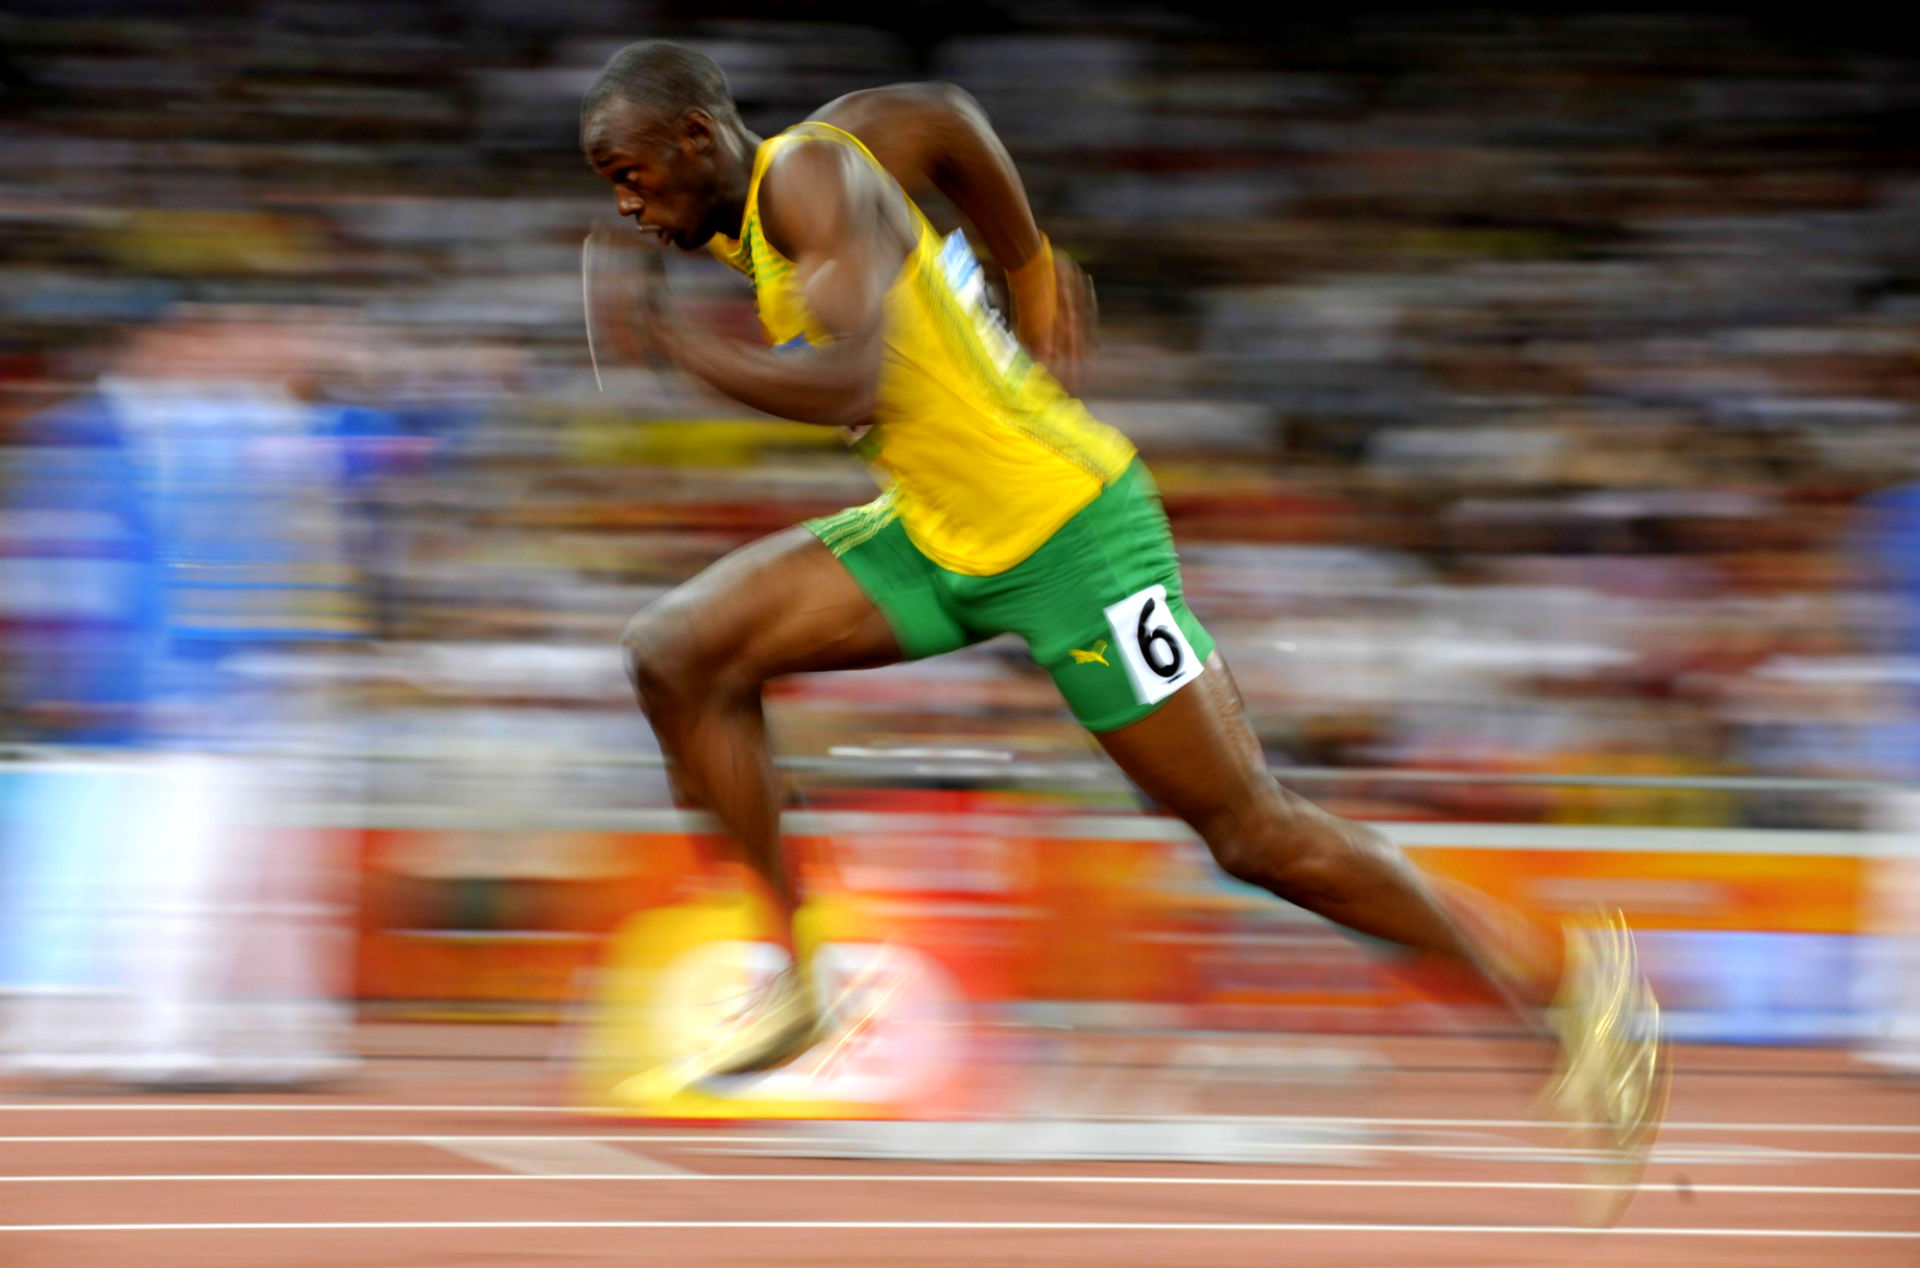
\includegraphics[scale=0.053]{bolt.png}\\
       \end{block}
  $\Downarrow$ (Validation)
      \begin{block}{Mathematical Model}
       \center
       $\frac{d^2x(t)}{dt^2} = \frac{F}{M}$\\
      \end{block}
  $\Downarrow$ (Verification)
  \begin{block}{Numerical Representation}
   \center
   $\frac{d^2x}{dt^2} = f''(t) = \frac{f(t+h) - 2 f(t) + f(t-h)}{h^2}$
   \end{block}
 \end{center}
\end{frame}

%===============================================================================
% why we care about mms/verification
%===============================================================================
\begin{frame}
  \frametitle{Why Verify?}
  \begin{block}{Reinhart and Kenneth S. Rogoff: Growth in a Time of Debt, 2010}
    \begin{itemize}
    \item ``Our main result is that whereas the link between growth and
	  debt seems relatively weak at $B!H(Bnormal$B!I(B debt levels, median
	  growth rates for  \textcolor{red}{countries with public debt
	  over roughly 90 percent of GDP are about one percent lower}
	  than otherwise'' 
     \item Dataset: ``inflation and GDP growth across varying levels
	   of debt for 20 advanced countries over the period 1946
	   through 2009''
     \item Rogoff testified in front of the Senate Budget Committee 
   \end{itemize}
  \end{block}
  \begin{block}{Inform Decision Makers}
    \begin{itemize}
     \item France: 30 Billion Euros in Austerity Measures
     \item England: 11.5 Billion Pounds in Austerity Measures
     \item ``Spain's national budget cuts of almost 14 percent
	   and regional budget cuts of up to 10 percent in health and
	   social services''
    \end{itemize}
  \end{block}
 
\end{frame}

%===============================================================================
% why we care about mms/verification
%===============================================================================
\begin{frame}
  \frametitle{Verification Failure}
  \begin{block}{Excel Error!}
    \begin{itemize}
     \item ``Instead of AVERAGE(L30:L49), AVERAGE(L30:L44) was used.''
     \item When corrected, GDP/DEBT ratios above 90\% had growth of 2.2\%
    \end{itemize}
  \end{block}

 \begin{center}
  \center
  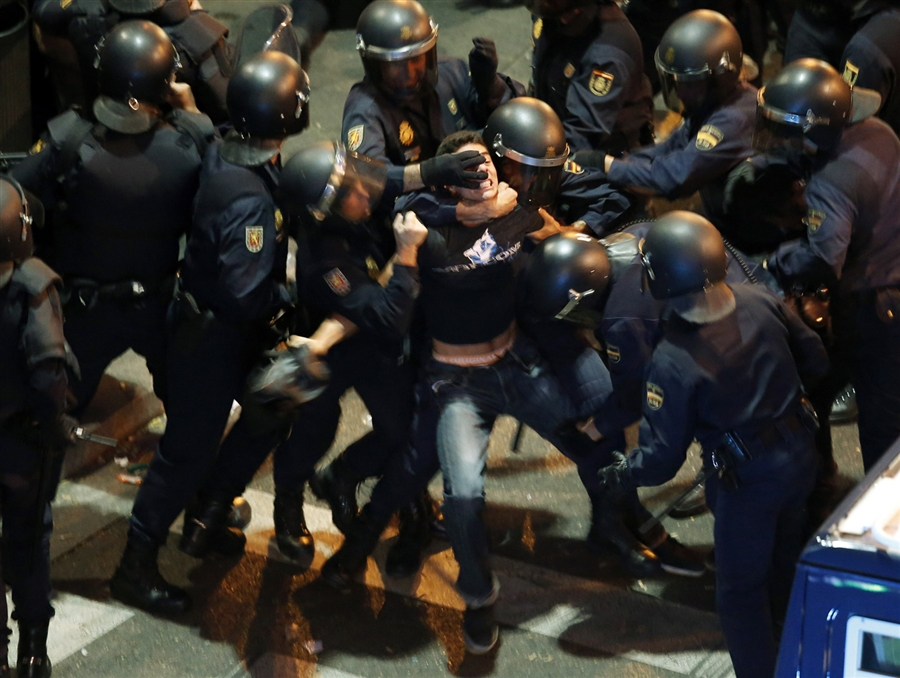
\includegraphics[scale=0.3]{riot.png}\\
 \end{center}
 
\end{frame}

%===============================================================================
% why we care about mms/verification
%===============================================================================
\begin{frame}
  \frametitle{JP Morgan needs more verification}
  \begin{block}{Estimating risk with computer models}
    \begin{itemize}
     \item JPMorgan$B!G(Bs CIO needed a new value-at-risk (VaR) model for the synthetic credit portfolio 
     \item ''London-based quantitative expert, mathematician and model developer`` was dispatched
     \item The model underestimated downside in portfolio
     \item Resulted in \$6 billion in losses and another \$600 million in fines.
    \end{itemize}
  \end{block}

  \begin{block}{What went wrong?}
    \begin{itemize}
     \item After subtracting the old rate from the new rate, the spreadsheet divided by their sum instead of their average
     \item The errors stemmed from a combination of copy-paste mistakes and a faulty equation created to crunch the numbers.
     \item This error likely had the effect of muting volatility by a factor of two!!
    \end{itemize}
  \end{block}
 
\end{frame}


%===============================================================================
% why we care about mms/verification
%===============================================================================
 \begin{frame}
   \frametitle{Surely those were isolated events, right?}
  \begin{block}{Other examples}
    \begin{itemize}
    \item Mars Surveyor (metric versus english units)
    \item Sleipner A - North Sea Oil Platform Collapse (``serious error in the finite element analysis'')
    \item Therac-25 (overdosed more than two-dozen patients with gamma radiation)
    \item Patriot missile mistiming (only off by one third of a second!)
    \end{itemize}
    \end{block}
 \end{frame}

%===============================================================================
% PECOS introductions: why we care about mms/verification
%===============================================================================
\begin{frame}
  \frametitle{Direct Numerical Simulations}

      \begin{block}{Physics Simulation}
        \begin{itemize}
	 \item 225 Billion Degrees of Freedom
	 \item 524,288 Processing Cores
	 \item 275 Million Compute Hours
	 \item Indistinguishable from physical experiments

          % this is when we put on our babuska hat and ask about blueprints
	 \item {\bf Are we confident in our predictions?}
          % maybe reference last slide: how right are we?
        \end{itemize}
      \end{block}
 \begin{center}
  \center
  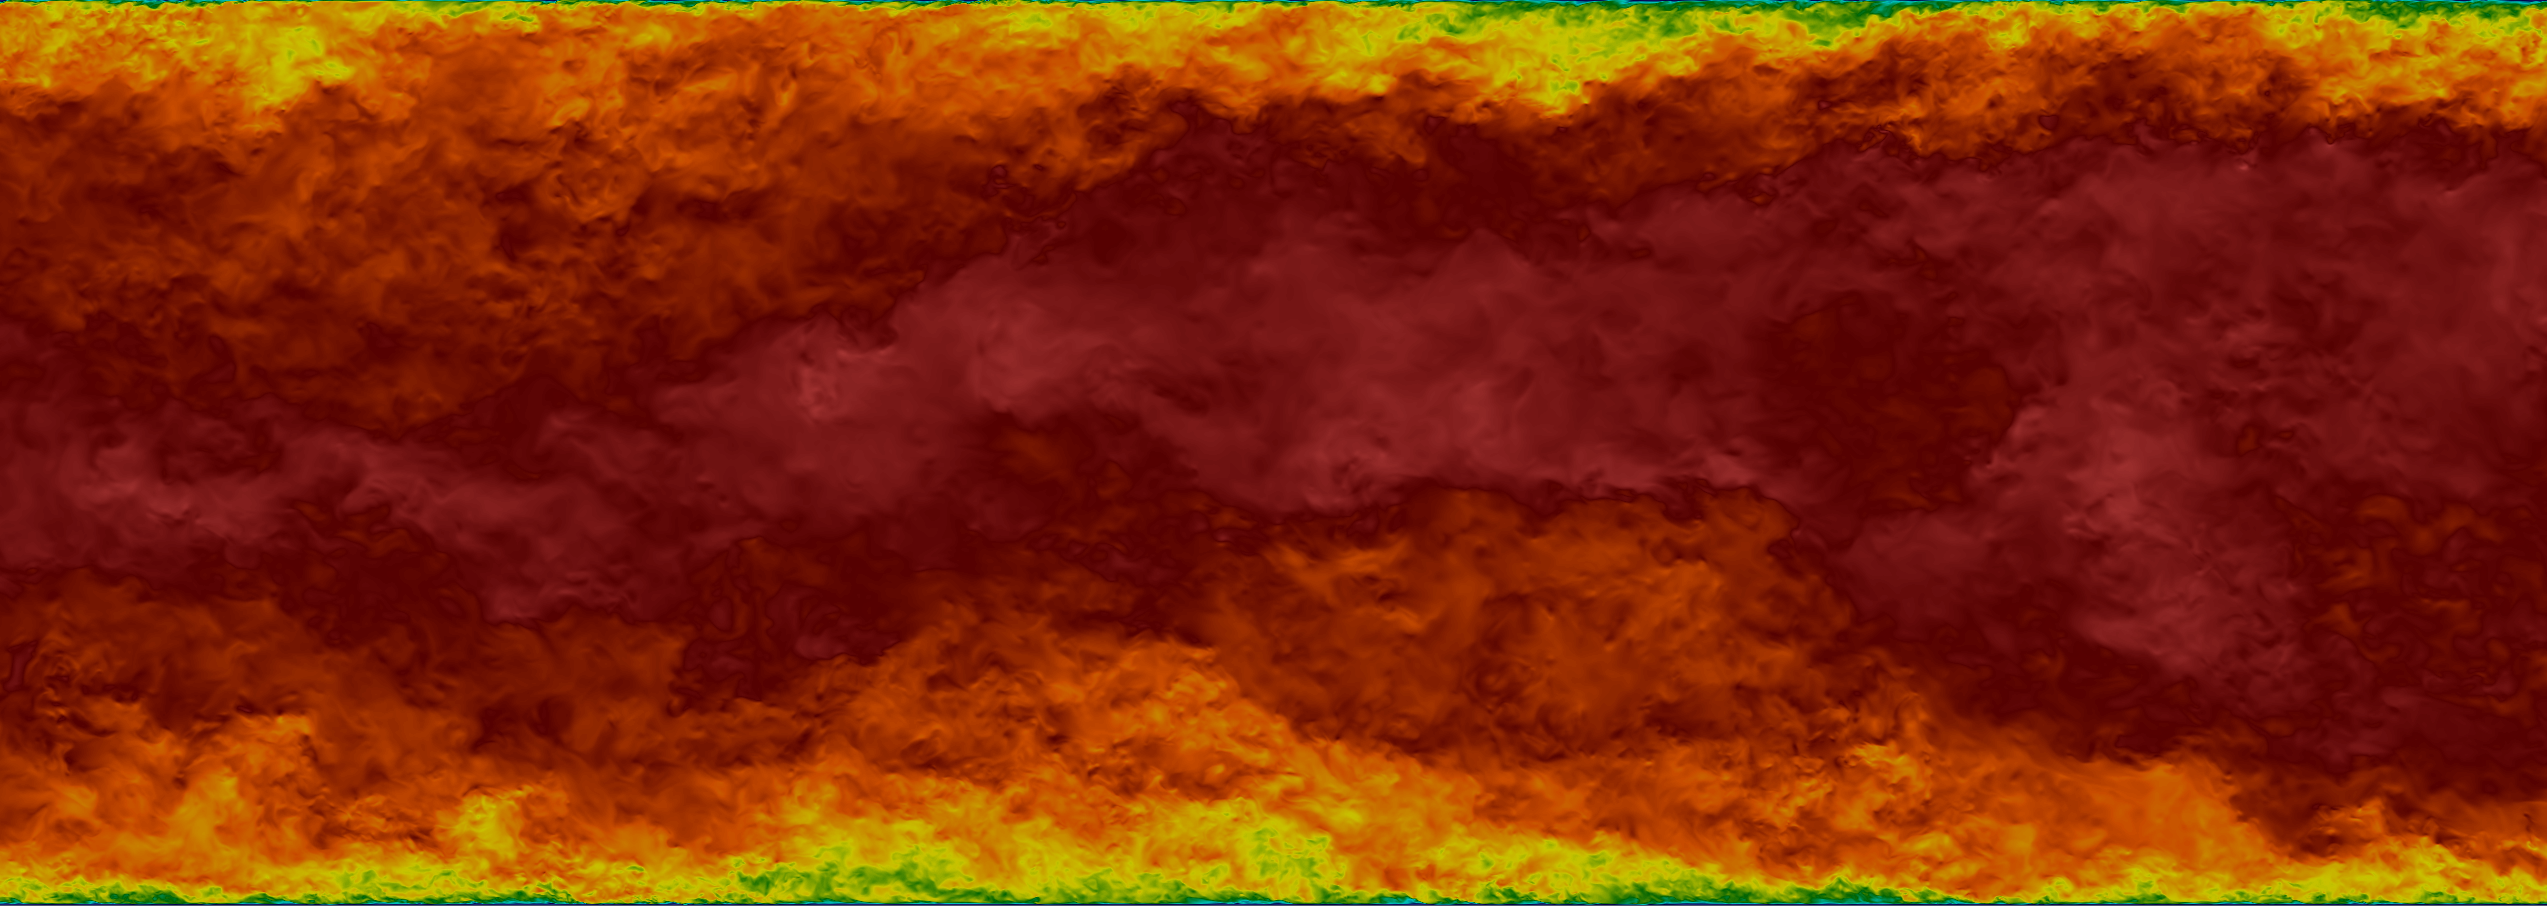
\includegraphics[scale=0.1]{channel.png}\\
 \end{center}
\end{frame}

%===============================================================================
% PECOS introductions: why we care about mms/verification
%===============================================================================
\begin{frame}
  \frametitle{Direct Numerical Simulations}

      \begin{block}{It's not you, it's me.}
        \begin{itemize}
	 \item ``We have released Mira for use.  However, service is degraded. Several
	       racks (1024 nodes each) remain offline, and the system will have a high
	       risk of hardware errors.''
	 \item ``A new efix was installed on Mira and Cetus which contains
	       fixes and performance enhancements for the BG/Q MPI and
	       PAMI packages.  All users are strongly advised to
	       recompile and relink their code.''
	 \item {\bf Are we STILL confident in our predictions?}
          % maybe reference last slide: how right are we?
        \end{itemize}
      \end{block}
 \begin{center}
  \center
  
\includegraphics[scale=0.08]{vor.png}\\
 \end{center}
\end{frame}


%===============================================================================
% verification
%===============================================================================

\begin{frame}
  \frametitle{Verification}

  \begin{block}{Verification of Scientific Software}
    \begin{itemize}
    \item Verification ensures that the outputs of a computation accurately reflect the solution of the mathematical models.
     %\item Essentially, we are testing if we have correctly instantiated mathematical equations in our code.
    \end{itemize}
  \end{block}

  % we probably want to have a spiffy example of what these mean, to avoid confusing our listeners
  \begin{block}{Code Verification}
    \begin{itemize}
    \item Ensuring that the code used in the simulation correctly
	  implements the intended numerical discretization of the model.
	  \begin{itemize}
	   \item This concept is *not* unique to Scientific Software 
	  \end{itemize}
    \end{itemize}
  \end{block}

  \begin{block}{Solution Verification}
    \begin{itemize}
    \item Are the errors from the numerical discretization sufficiently small?
    \item Is the convergence rate consistent with the numerical scheme?
	     %\begin{itemize}
     % \item Is the numerical solution to a set of model equations ``close enough'' to the exact solution?
	      %     \end{itemize}
    \end{itemize}
  \end{block}
  
\end{frame}

%===============================================================================
% solution verification
%===============================================================================

\begin{frame}
  \frametitle{Solution Verification Methods}

  \begin{block}{Method of Exact Solutions}
    \begin{itemize}
      \item Numerically solve the governing equations for which the solution can be determined analytically.
    \end{itemize}
  \end{block}
  
  \begin{block}{MMS}
    \begin{itemize}
    \item Often, analytical solutions either:
    \begin{itemize}
      \item Do not exist (Navier-Stokes)
      \item Do not fully exercise equations (e.g. a symmetric
	solution, nonlinearities)
    \end{itemize}
    \item Alleviate this using Method of Manufactured Solutions (MMS)
      \begin{itemize}
      \item  Simply put, we ``create'' our own solutions
      \end{itemize}
    \end{itemize}
  \end{block}
  
\end{frame}

%===============================================================================
% add slide about laplace equation solution here
%===============================================================================

\begin{frame}
  \frametitle{Manufactured solution to Laplace's Equation}
  
  Laplace's Equation:
  \begin{equation}
      \nonumber      
    \nabla^2 \phi = 0
  \end{equation}
  In two dimensions:
  \begin{equation}
      \nonumber      
    \frac{\partial^2 \phi}{\partial x^2} + \frac{\partial^2 \phi}{\partial y^2} = 0
  \end{equation}
  \newline
  \newline
  ``Manufacture'' a solution, with two constants:
  \begin{equation}
      \nonumber
    \phi(x,y) = (\textcolor{red}{Ly}-y)^2 (\textcolor{red}{Ly}+y)^2 + (\textcolor{red}{Lx}-x)^2 (\textcolor{red}{Lx}+x)^2
  \end{equation}  

\end{frame}

%===============================================================================
% calculate the source term
%===============================================================================

\begin{frame}
  \frametitle{Calculating the Source Term}

  We insert our manufactured solution back into the governing equations:
  \begin{equation}
      \nonumber
    \frac{\partial^2 ((Lx-x)^2 (Lx+x)^2)}{\partial x^2} + \frac{\partial^2 ((Ly-y)^2 (Ly+y)^2)}{\partial y^2} = 0
  \end{equation}

  \begin{equation}
    \begin{split}
      \nonumber      
      = & 2(Lx-x)^2 - 8(Lx-x)(Lx+x)+2(Lx+x)^2 \\
      + & 2(Ly-y)^2 - 8(Ly-y)(Ly+y)+2(Ly+y)^2 \\
      \textcolor{red}{\neq} & \textcolor{red}{0}
    \end{split}
  \end{equation}
  This does not satisfy Laplace's Equation!
  \newline
  \newline
  \begin{block}{}
    To balance the equation, add the residual to the RHS as a source term. 
  \end{block}
\end{frame}

%===============================================================================
% back to laplace: we have a solution, now what do we do with it?
%===============================================================================
\begin{frame}
  \frametitle{Example Verification Use Case}
  \begin{block}{}
    To solve Laplace's Equation numerically, we need a discretization scheme.
  \end{block}
  Let's use a 2nd order finite central difference:
  \begin{equation}
      \nonumber      
    \phi_i'' \approx \frac{\phi_{i+1} - 2\phi_{i} + \phi_{i-1}}{h^2} + O(h^2)
  \end{equation}
  This requires solving the implicit system of equations: 
  \begin{equation}
      \nonumber      
      A \vec \phi = \textcolor{red}{f}
  \end{equation}
   You can use your favorite linear solver (e.g. PETSc) to solve the
   system.
 %, or we'll provide a simple (slow) Gauss-Seidel iterative example.
%  We will use a conjugate gradient solver to invert the matrix A.

\end{frame}


%===============================================================================
% back to laplace: we have a solution, now what do we do with it?
%===============================================================================

 \begin{frame}
   \frametitle{Problem: Solve 2D Laplacian using Finite-Differencing}

   \begin{block}{Outline}
     \begin{itemize} 
     \item Write a program in C/C++, F90, Python, etc. 
     \item {\em Inputs}: 
       \begin{itemize}
	 \item \# of points in one direction ({\em npts})
	 \item the physical dimension of one side ($L_x$, $L_y$)
       \end{itemize}
     \item {\em Output}: $l_2$ error between your numerical solution
       and an exact solution derived from a manufactured solution
       \begin{equation}
         \nonumber
         l_2 = \sqrt{ \frac{\sum_{i=1}^{\text{\tiny N}} (\phi_i-\phi_i^{\text{\tiny exact}})^2}N}
       \end{equation}
     \item {\em Runs}: Run your snazzy code for $\text{npts} =
       5,9,17,\text{and } 33$ and plot $l_2$ norm as a function of $1/h$ where
       $h=\text{length}/(\text{npts}-1)$
       
     \end{itemize}    
   \end{block}

 \end{frame}

%===============================================================================
% convergence plot
%===============================================================================
\begin{frame}
  \frametitle{Example Results: What we're hoping for}
  2nd Order Central Finite-difference Scheme

 \begin{center}
  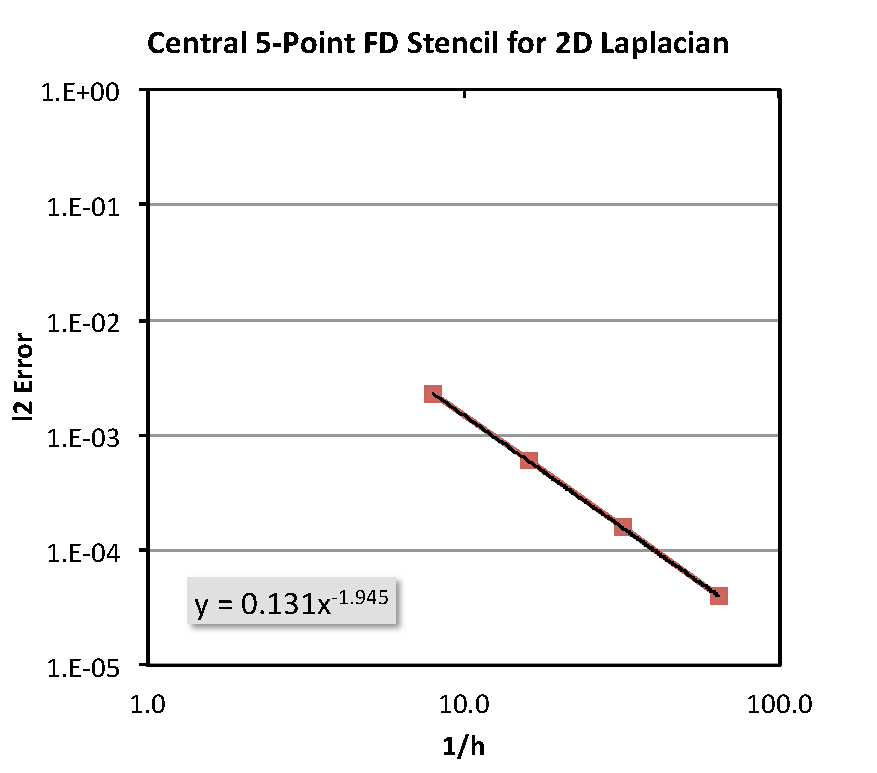
\includegraphics[width=0.7\linewidth]{laplace_central_diff2}
 \end{center}
  
\end{frame}


%% %===============================================================================
%% % fix bug
%% %===============================================================================
 \begin{frame}
   \frametitle{This Process Finds Bugs}
      \begin{center}
        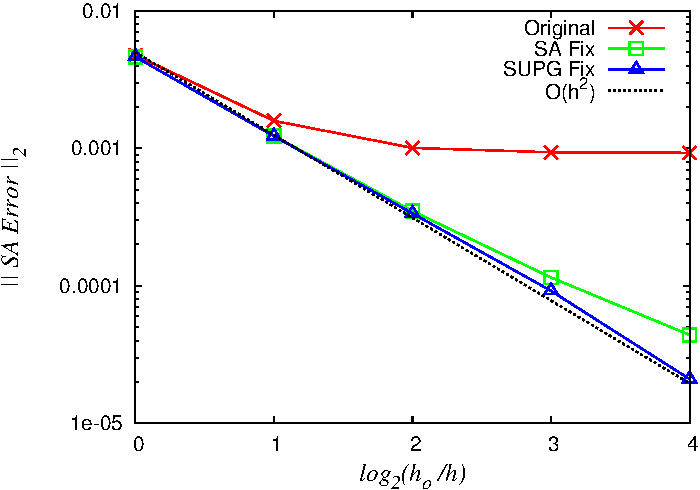
\includegraphics[scale=.8]{mms_grid_convergence.pdf} \\
      \end{center}

 \end{frame}

%% %===============================================================================
%% % code looks good, compare solutions, is this 'enough'? 
%% %===============================================================================
%% \begin{frame}
%%   \frametitle{code looks good}

%%   but need some metric to be sure it 'is' good--- compare solutions under mesh refinement

%% \end{frame}
%% % now we need to introduce concept of mesh refinement
%% % and have a plot of mesh refinement


%===============================================================================
% Is this useful? -- show how this technique helped us find a bug
%===============================================================================
\begin{frame}
  \frametitle{Useful for Detecting \textcolor{red}{Subtle} Bugs}

  \begin{columns}[c]
    \begin{column}{6cm}

      \begin{block}{Verification of FIN-S}
        \small
        \begin{itemize}
        \item \small FANS, Spalart-Allmaras
          
        \item Derivative:
        \end{itemize}
          \begin{equation}
            \nonumber  
            \frac{d(sa)}{dx} = \frac{1}{\rho}*\left(\frac{d(\rho *sa)}{dx} - sa \frac{d\rho}{dx}\right)
          \end{equation}
          
        \begin{itemize}
        \item In code:
        \end{itemize}

          \begin{equation}
            \nonumber  
            \frac{d(sa)}{dx} = \frac{1}{\rho}*\frac{d(\rho *sa)}{dx} - sa \frac{d \rho}{dx}
          \end{equation}
          
      \end{block}
    \end{column}
   
   % achtung! update me!
    \begin{column}{5cm}
      \begin{center}
        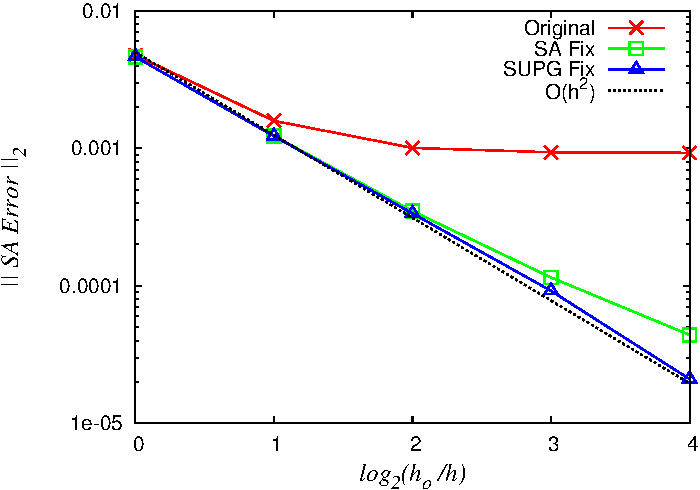
\includegraphics[scale=.45]{mms_grid_convergence.pdf} \\
      \end{center}
    \end{column}

    \end{columns}

\end{frame}

%===============================================================================
% maple
%===============================================================================
\begin{frame}
 \frametitle{Summary}
  \begin{block}{What we have learned:}  
   \begin{itemize}
    \item We can generate MS even for systems we do not have solutions for
    \item The MMS is a powerful method to verify rates of convergence
    \end{itemize}
  \end{block}
  \begin{block}{\textcolor{red}{Why is this not more commonly done?}}
   \begin{itemize}
    \item Solution Generation is complex and time intensive
    \item Meaningful Solution generation can be subtle
    \end{itemize}
  \end{block}


\end{frame}

%===============================================================================
% maple
%===============================================================================
\begin{frame}
  \frametitle{A Real Example}
  \begin{block}{MMS Creation Process}
    \begin{itemize} 
      \small
      \item Start by ``manufacturing'' a suitable closed-form exact solution
      \item For example, the 10 parameter trigonometric solution of the form: 
        \newline(Roy, 2002)
        \small
        \begin{equation}
          \begin{split}
            \nonumber
            \ms (x,y,z,t) = \textcolor{red}{\ms_0}  &+  \textcolor{red}{\ms_x}\, f_s \left(\frac{\textcolor{red}{a_{\ms x}} \pi x}{\textcolor{red}{L}} \right) +  \textcolor{red}{\ms_y} \,f_s\left(\frac{\textcolor{red}{a_{\ms y}} \pi y}{\textcolor{red}{L}}\right) +\\
            & +  \textcolor{red}{\ms_z} \,f_s\left(\frac{\textcolor{red}{a_{\ms z}} \pi z}{\textcolor{red}{L}}\right)+ \textcolor{red}{\ms_t} \,f_s\left(\frac{\textcolor{red}{a_{\ms_t}} \pi t}{\textcolor{red}{L}}\right)
          \end{split}
        \end{equation}
        \normalsize
      \item Apply this solution to equations of interest, solve for source terms (residual)
    \end{itemize}
  \end{block}  
  \normalsize
  Accomplished using packages such as Maple, Mathematica, SymPy,
 Macsyma, etc.
\end{frame}

%===============================================================================
% maple MMS example
%===============================================================================
\begin{frame}
  \frametitle{Maple MMS: 3D Navier-Stokes Energy Term}

  \begin{center}
    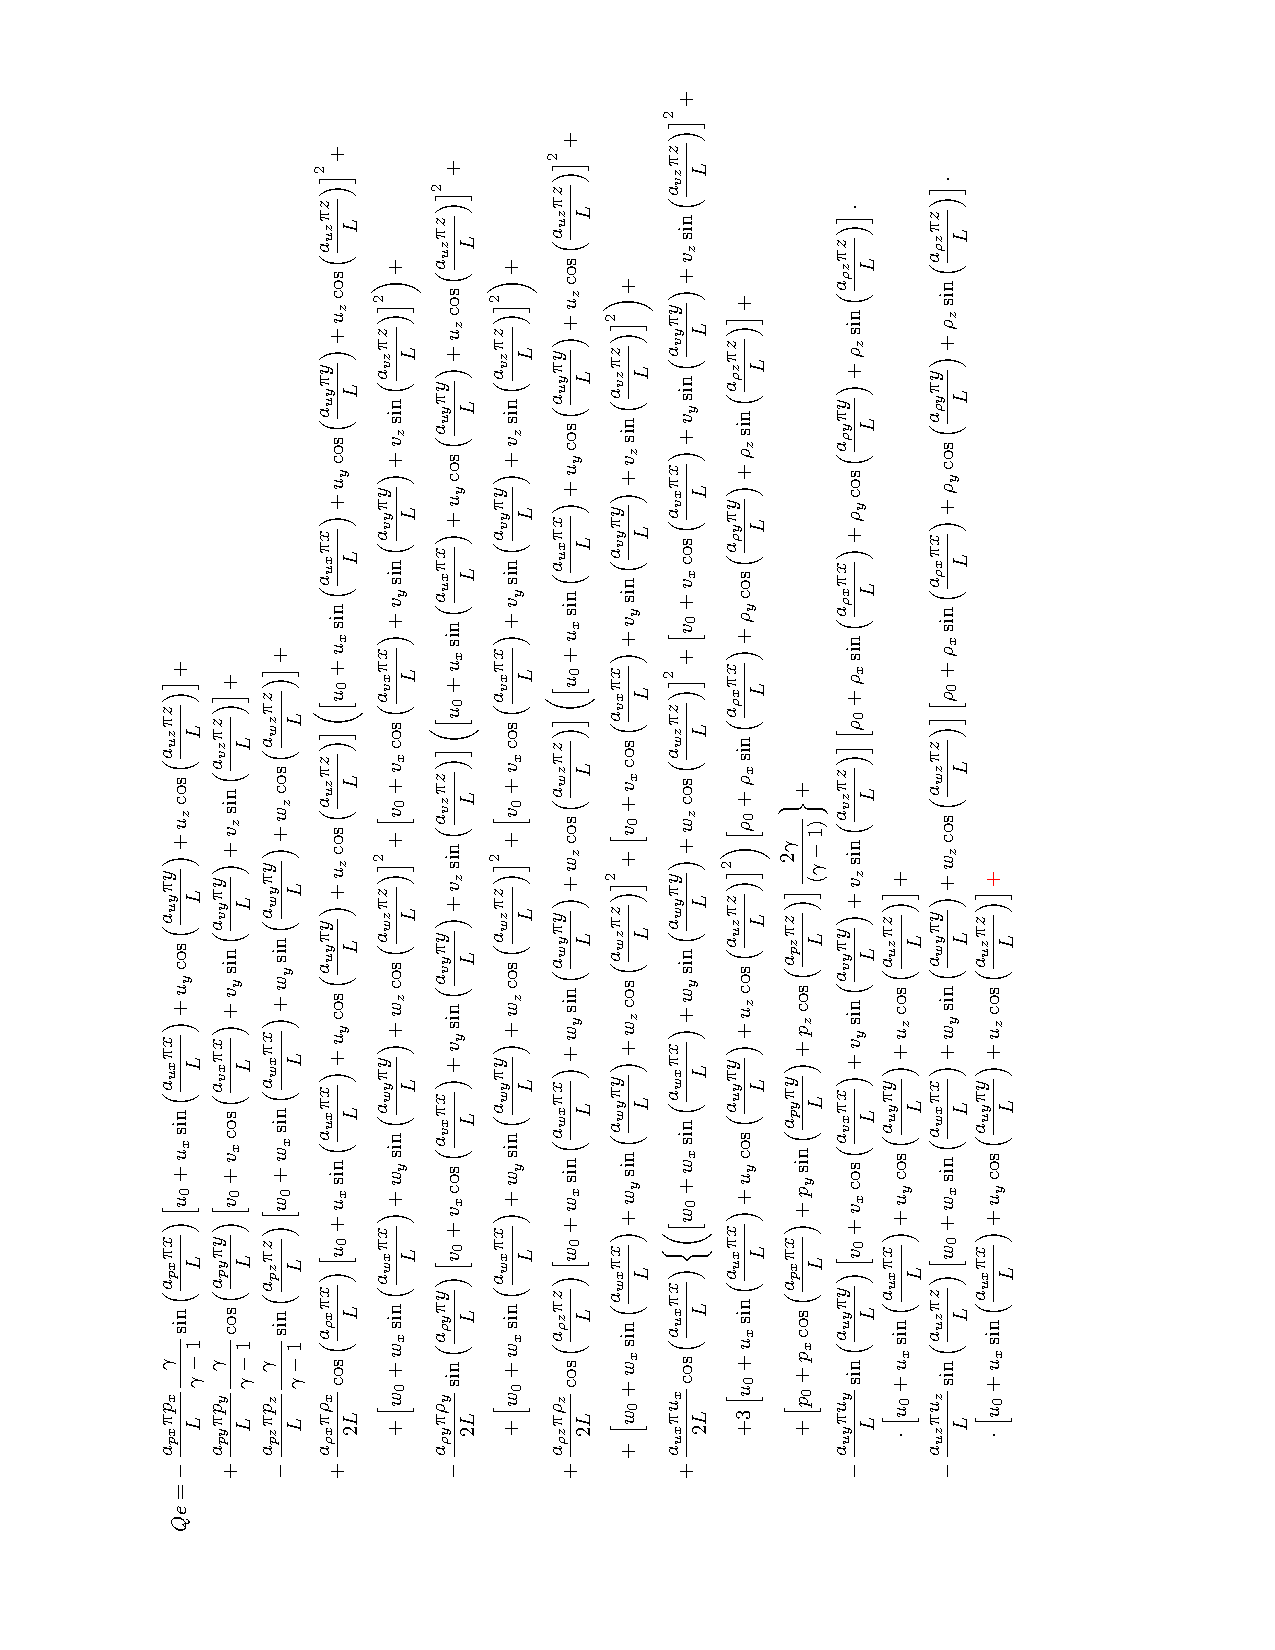
\includegraphics[scale=0.4,angle=-90]{page1}  
  \end{center}

\end{frame}
%===============================================================================
% maple MMS example
%===============================================================================
\begin{frame}
  \frametitle{But wait, there's more!}

   \begin{center}
     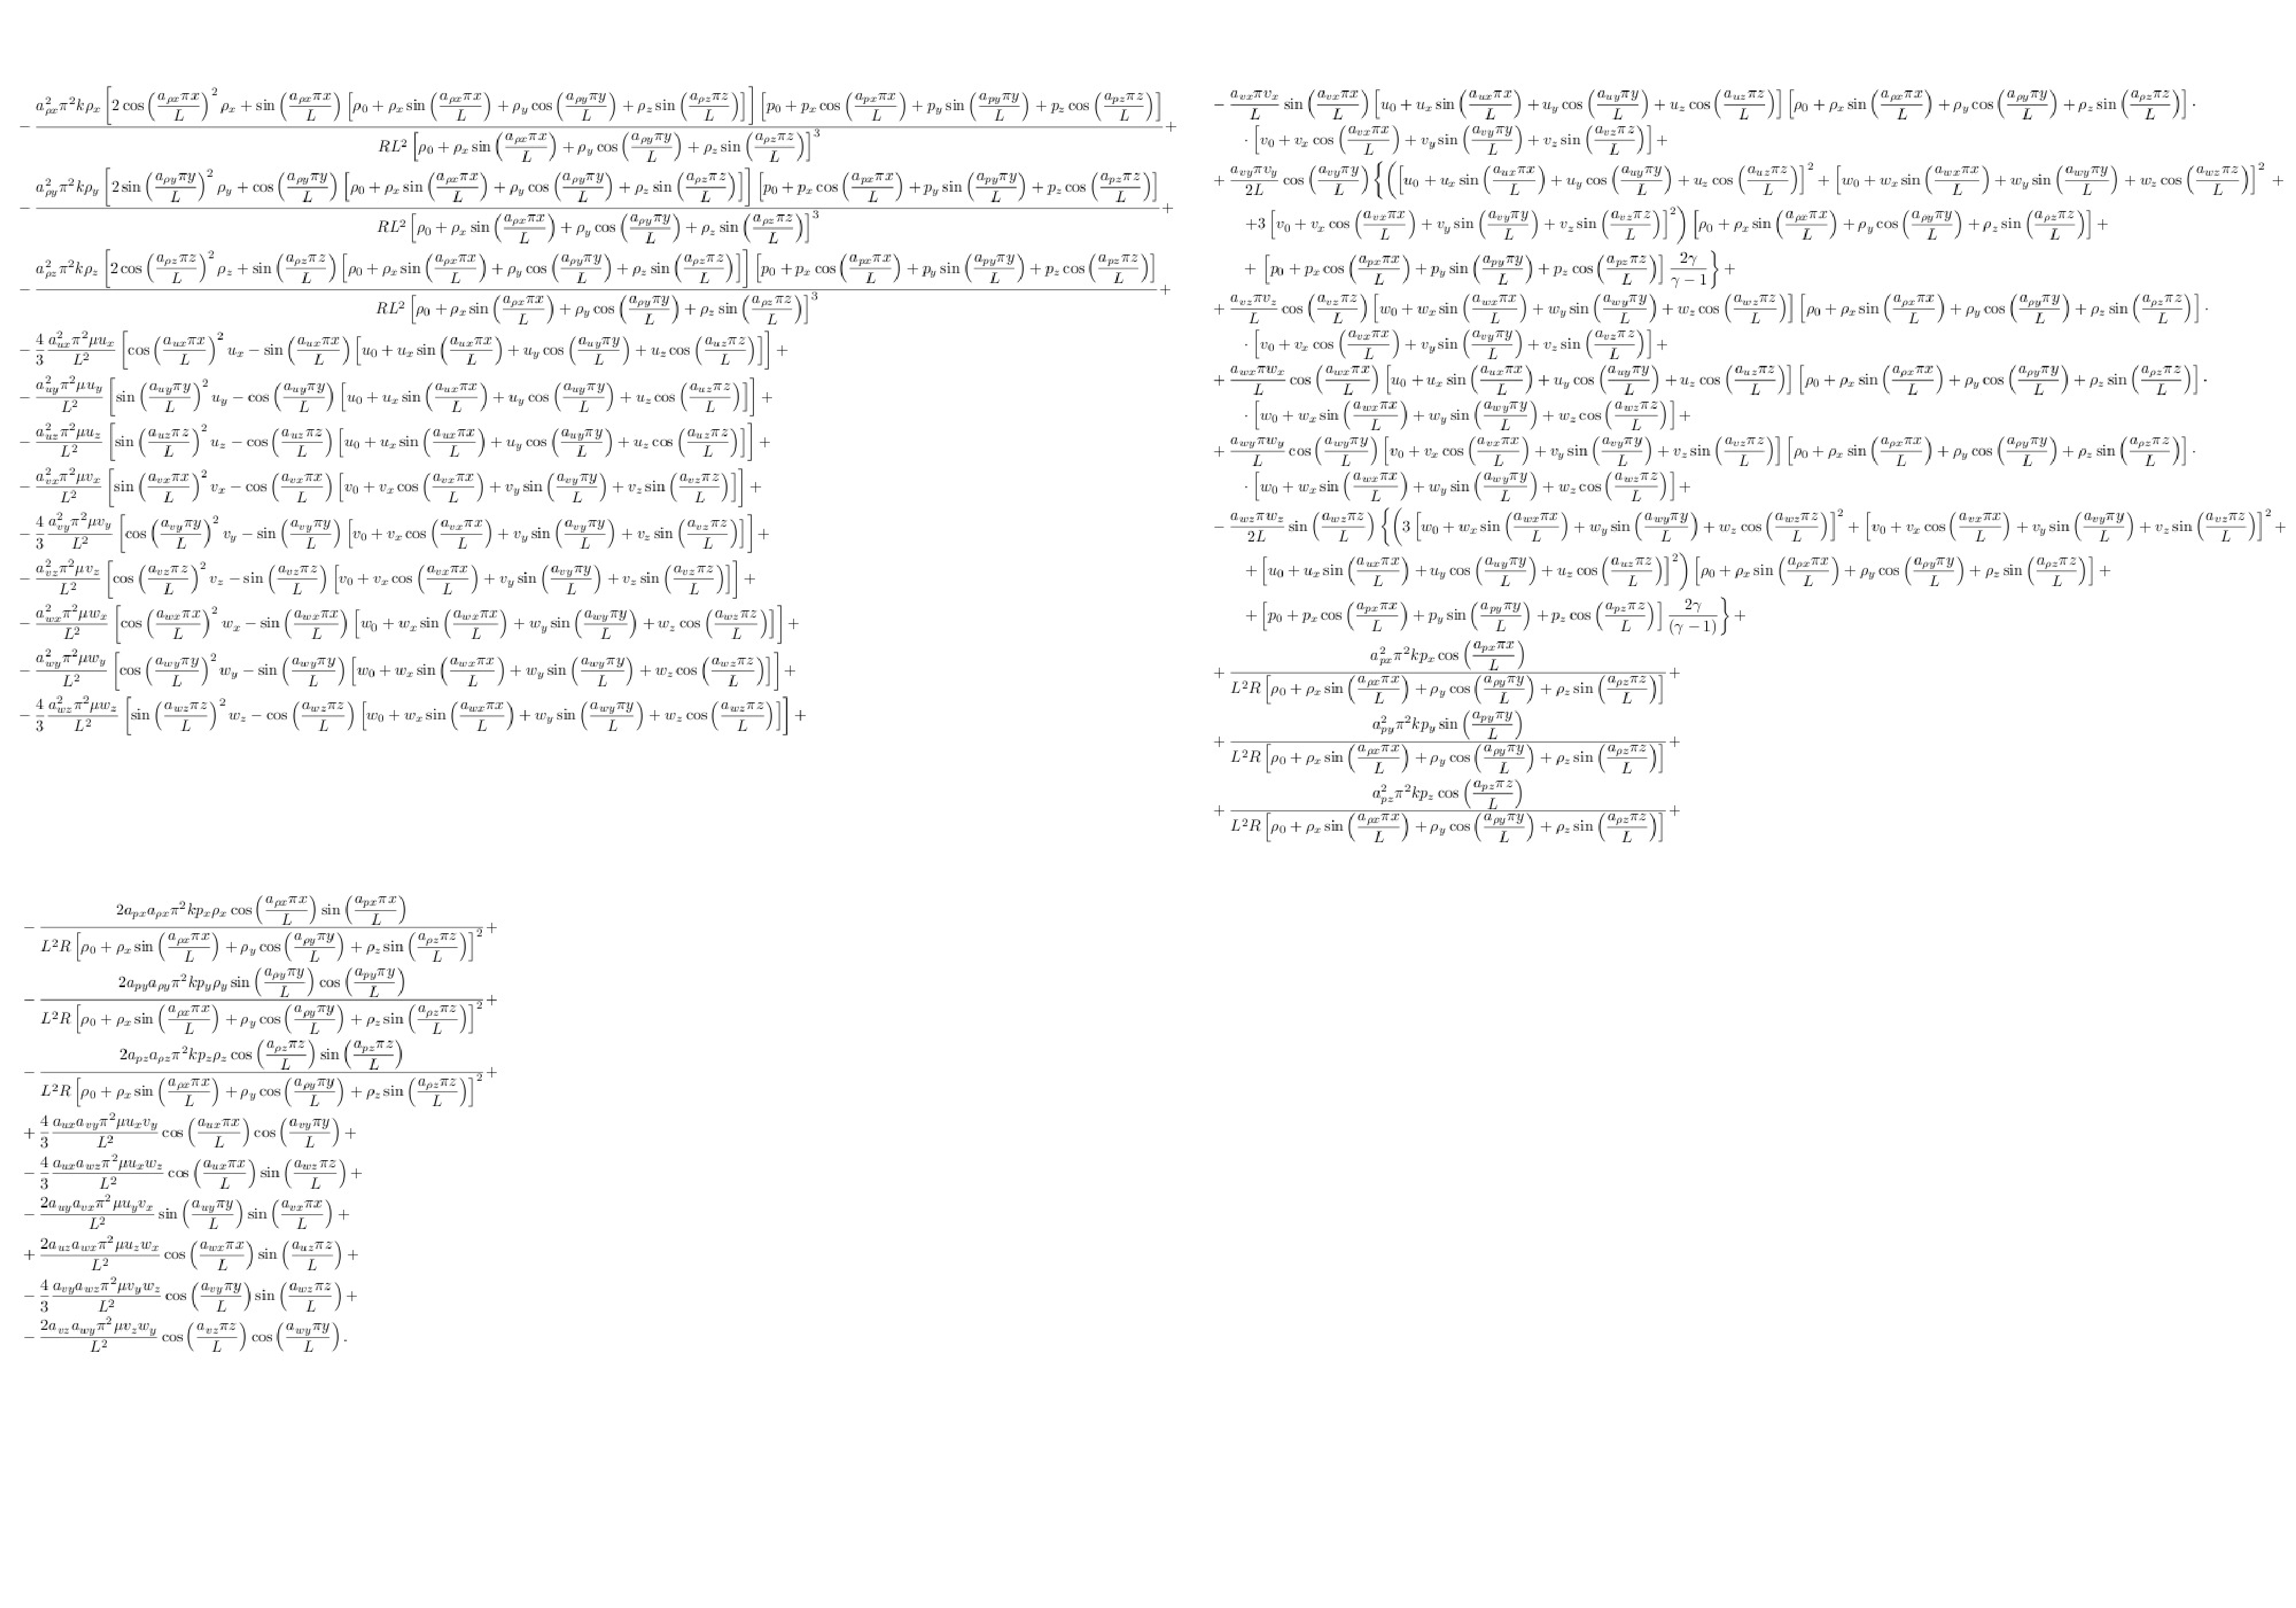
\includegraphics[scale=0.17]{maple}
   \end{center}

\end{frame}

%===============================================================================
% c_code
%===============================================================================

\begin{frame}
  \frametitle{C-code output}
  \center
  \vspace{-15pt}
  \hspace{-1cm}\quad
  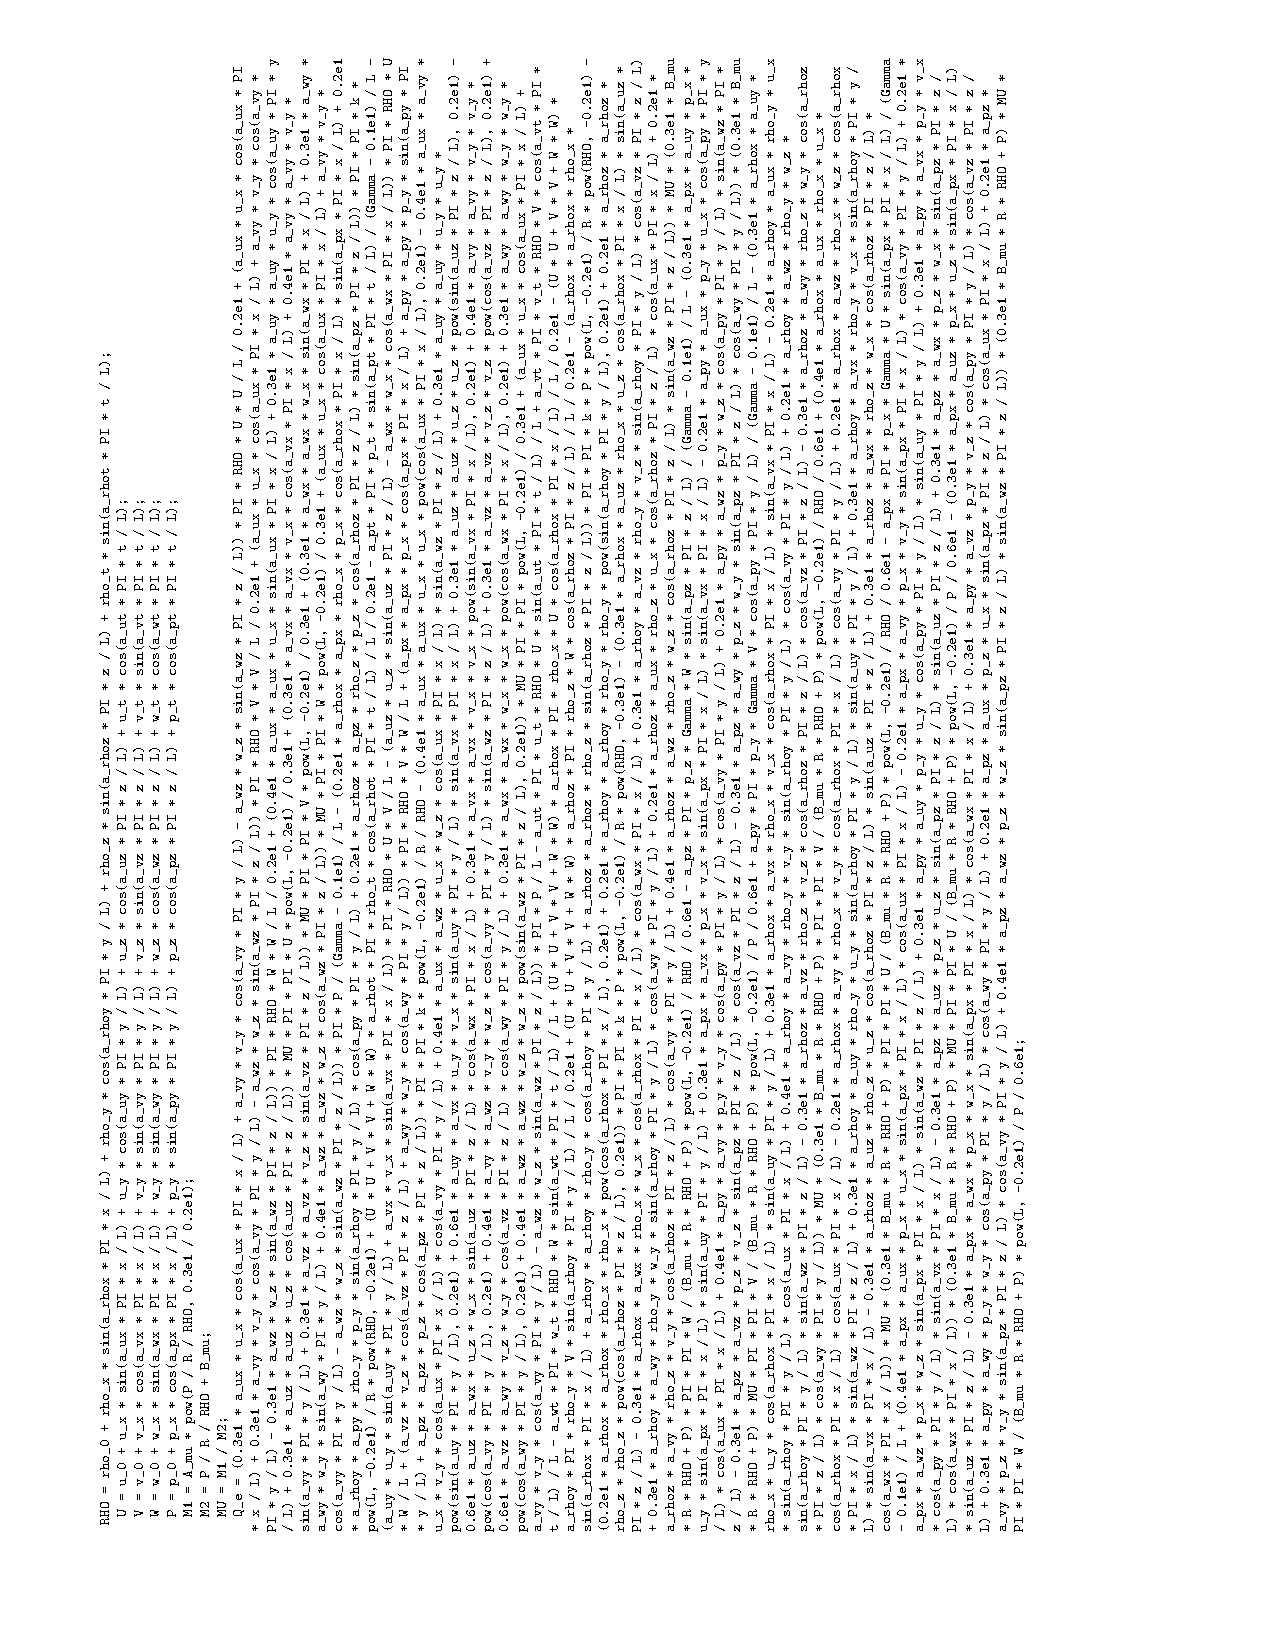
\includegraphics[scale=0.40]{EnergySutherland_3d}  
\end{frame}

%===============================================================================
% achtung! add modeling talk from SIAM and AIAA here!
%===============================================================================

\begin{frame}
  \frametitle{Meaningful Verification is difficult}

 \begin{block}{What Constitutes a Robust Test?}
  \begin{itemize}
   \item How ``strong'' is a verification test for a particular codebase?
	 \begin{itemize}
	  \item Can you characterize your confidence in a codebase?
	  \item What constitutes a strong test?
	 \end{itemize} 
  \end{itemize}
 \end{block}

 \begin{block}{Verification Metrics}
  \begin{itemize}
   \item In general, you cannot ``verify'' a codebase
   \begin{itemize}
    \item You can, however, detect {\bf verification failures}
   \end{itemize}
  \end{itemize}
 \end{block}

  \begin{block}{Physically-based MS}
   \begin{itemize}	   
    \item Exercise each term in the PDE in a similar way to that of a
	  real solution	
   \end{itemize}
  \end{block}

\end{frame}

%===============================================================================
% intro to AIAA 
%===============================================================================
\begin{frame}
 \frametitle{Example Problem}

 \begin{block}{Complex Codebase}
  \begin{itemize}
   \item Finite Element hypersonic code, fully implicit Navier-Stokes (FIN-S)
   \item Favre-Averaged Navier Stokes (FANS) + Spalart-Allmaras (SA)
	 turbulence model
  \end{itemize}
 \end{block}

  \begin{block}{FANS + SA}
  \tiny
  \begin{gather*}
   \pp{\bar{\rho}}{t} + \pp{}{x_i} (\bar{\rho}\tilde{u}_i) = 0 \\
   \pp{}{t} \left(\bar{\rho} \tilde{u}_i \right) + \pp{}{x_j}
   \left(\bar{\rho} \tilde{u}_j \tilde{u}_i  \right) = - \,
   \pp{\bar{p}}{x_i} + \pp{}{x_j}\left( 2 (\mu + \mu_t) \tilde{S}_{ji}
   \right) \\ 
   \pp{}{t} \left[ \bar{\rho} \left( \tilde{e} + \frac{1}{2} \tilde{u}_i
   \tilde{u}_i \right) \right] + \pp{}{x_j} \left[ \bar{\rho} \tilde{u}_j
   \left( \tilde{h} + \frac{1}{2} \tilde{u}_i \tilde{u}_i \right) \right]
   =  \pp{}{x_j} \left( 2 (\mu + \mu_t) \tilde{S}_{ji} \tilde{u}_i \right)
   + \pp{}{x_j} \left[ \left( \frac{\mu}{\Pr} + \frac{\mu_t}{\Pr_t}
   \right) \pp{\tilde{h}}{x_j} \right] \\ 
   \pp{}{t}(\bar{\rho} \sa) + \pp{}{x_j} (\bar{\rho} \tilde{u}_j \sa) =
   c_{b1} S_{\mathrm{sa}} \bar{\rho} \sa - c_{w1} f_w \bar{\rho} \left(
   \frac{\sa}{d} \right)^2 + \frac{1}{\sigma} \pp{}{x_k} \left[ (\mu +
   \bar{\rho} \sa) \pp{\sa}{x_k} \right] + \frac{c_{b2}}{\sigma}
   \bar{\rho} \pp{\sa}{x_k} \pp{\sa}{x_k}
  \end{gather*}
\end{block}
\end{frame}


%===============================================================================
% failures of other problems
%===============================================================================

\begin{frame}
 \frametitle{Insufficient Verification}

  \begin{block}{Shortcoming of other SA MS}
   \begin{itemize}
    \item Bond solution: sinusoidal, only satisfies no-slip.
    \item E\c{c}a solutions: noted to have a suboptimal rate of convergence
   \end{itemize}
  \end{block}	  

  \begin{center}
    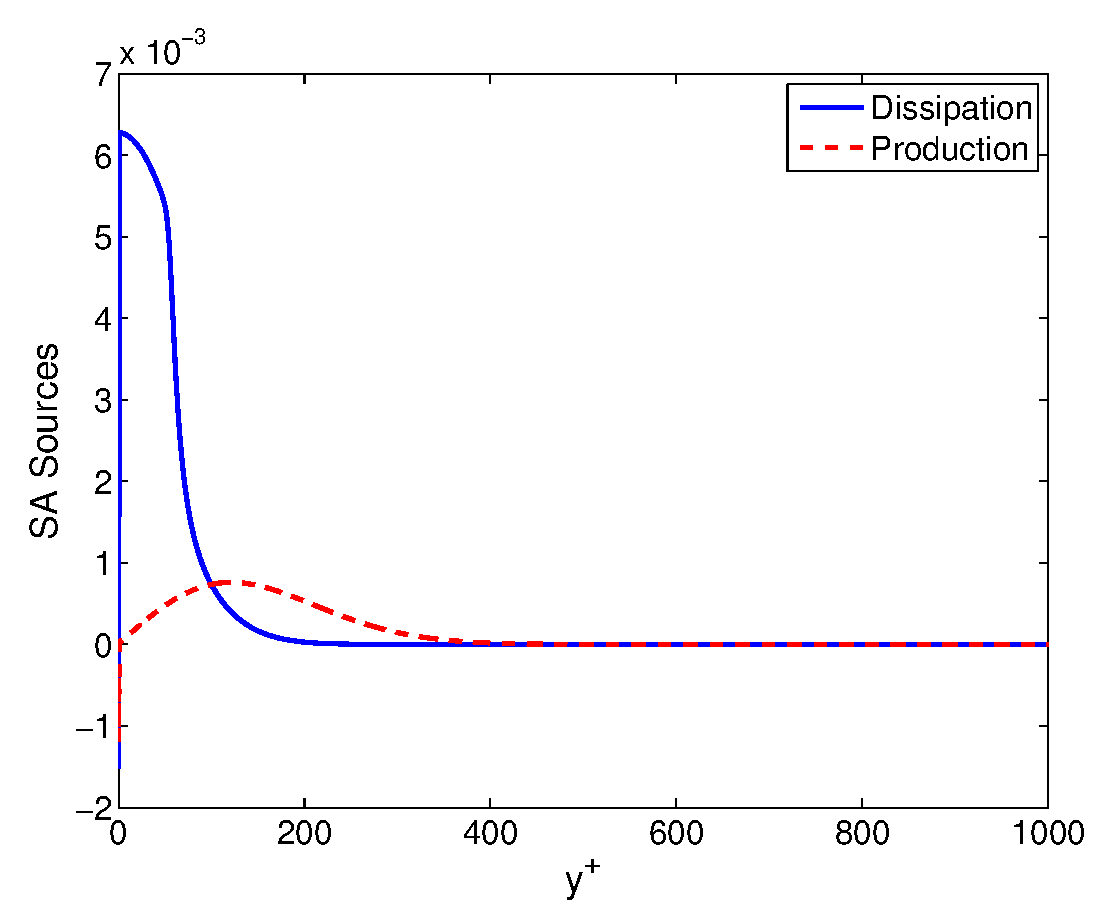
\includegraphics[width=.5\linewidth]{ms1_sources_1000} \\
  \end{center}

\end{frame}

%===============================================================================
% blow up the wall area
%===============================================================================

\begin{frame}
\frametitle{A Closer Look}

 \begin{block}{Shortcoming of other SA MS}
  \begin{itemize}
    \item E\c{c}a solutions are shown to have instabilities or near-wall
	  features that disrupt the correct rate of convergence 
   \begin{itemize}
    \item Offending term: $\nu_{sa} = \tilde
	  \nu_{\text{max}}\eta_{\nu}^2e^{1-\eta^2_{\nu}}$
   \end{itemize}
  \end{itemize}
 \end{block}

 \begin{center}
  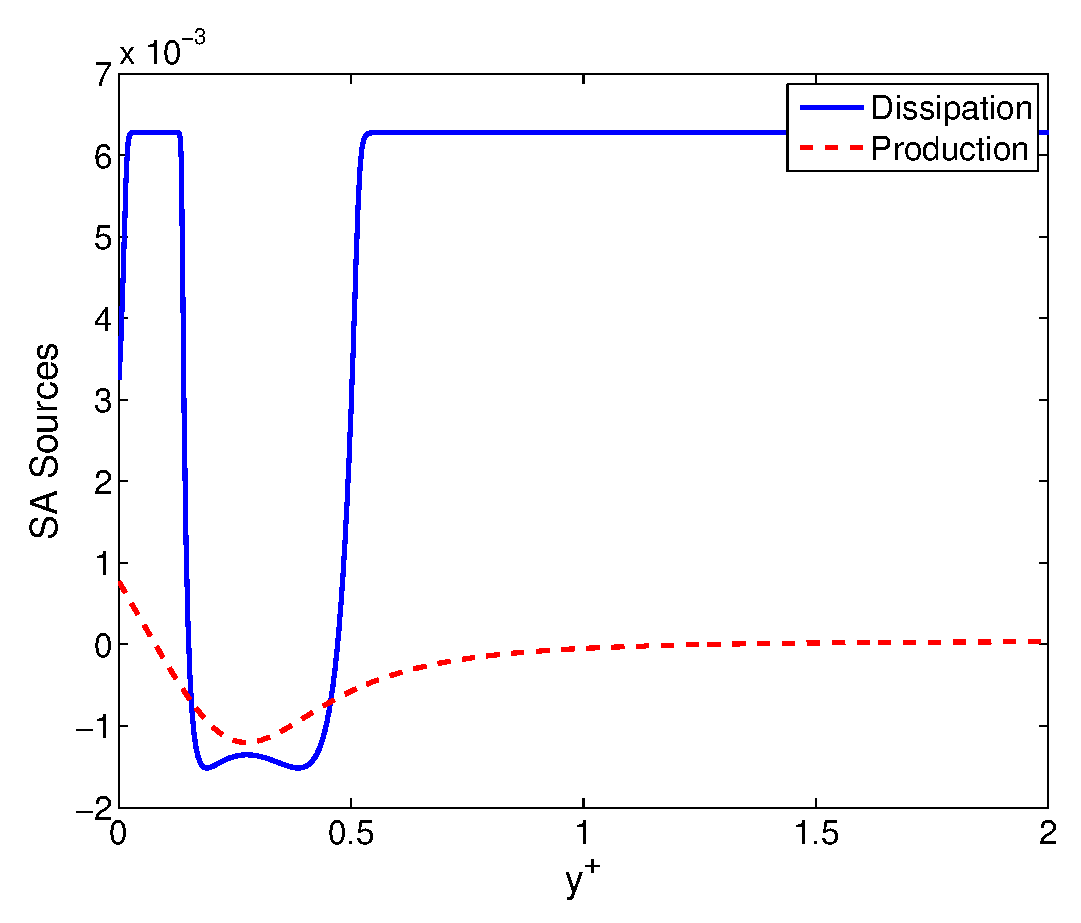
\includegraphics[width=.5\linewidth]{ms1_sources_2} \\
 \end{center}

\end{frame}

%===============================================================================
% our idea of SA
%===============================================================================
 \begin{frame}
   \frametitle{Our SA Manufactured Solution}

  \begin{block}{}
   \begin{itemize}

    \item Use our understanding of incompressible flow
	  physics to inform our modeling assumptions for this MS

   \end{itemize}
  \end{block}

  \begin{block}{Streamwise Velocity}
   \begin{itemize}
  
    \item The mean streamwise velocity is given by,
	  \begin{equation*}\label{eq:u_01}
	   \tilde{u} = \frac{\textcolor{red}{u_{\infty}}}{\textcolor{red}{A}} \sin \left( \frac{\textcolor{red}{A}}{\textcolor{red}{u_{\infty}}} u_{eq} \right)
	  \end{equation*}
	  
	  The van Driest equivalent velocity can be written as,
	  %
	  \begin{equation*}\label{eq:u_02}
	   u_{eq} = u_{\tau} u_{eq}^+ ,
	  \end{equation*}
	  
    \item Must specify both $u_{\tau}$ and $u^+_{eq}$
	  
   \end{itemize}
  \end{block}

 \end{frame}

%===============================================================================
% our idea of SA
%===============================================================================
 \begin{frame}
   \frametitle{Completing Streamwise Velocity Specification}
  

  \begin{block}{Correlations}
   \begin{itemize}

    \item Friction velocity can be determined from the skin friction coefficient

   \item The incompressible $1/7$th power law is used
	 for the skin friction coefficient.  Thus,
	 %
	 \begin{equation*}\label{eq:u_05}
	  c_{f,\texttt{inc}}(Re_x) = \textcolor{red}{C_{cf}} Re_{x}^{-1/7}
	 \end{equation*}
	 
   \item To complete the manufactured solution, $u^+_{eq}$ is set
	 using the velocity profile model of Cebeci and
	 Bradshaw (1980):
	 %
	 \begin{equation*}\label{eq:u_06}
	  u_{eq}^+ = \frac{1}{\textcolor{red}{\kappa}} \log \left( 1 + \textcolor{red}{\kappa} y^+ \right) + \textcolor{red}{C_1} \left[ 1 - e^{-y^+/\textcolor{red}{\eta_1}} - \frac{y^+}{\textcolor{red}{\eta_1}} e^{-y^+ \textcolor{red}{b}} \right]
	 \end{equation*}
    \end{itemize}
  \end{block}
 \end{frame}


%===============================================================================
% show how the solutions 'look'
%===============================================================================
 \begin{frame}
   \frametitle{Manufactured Velocity Profiles}

  \begin{columns}[c]
    \begin{column}{5cm}
    \begin{center}
     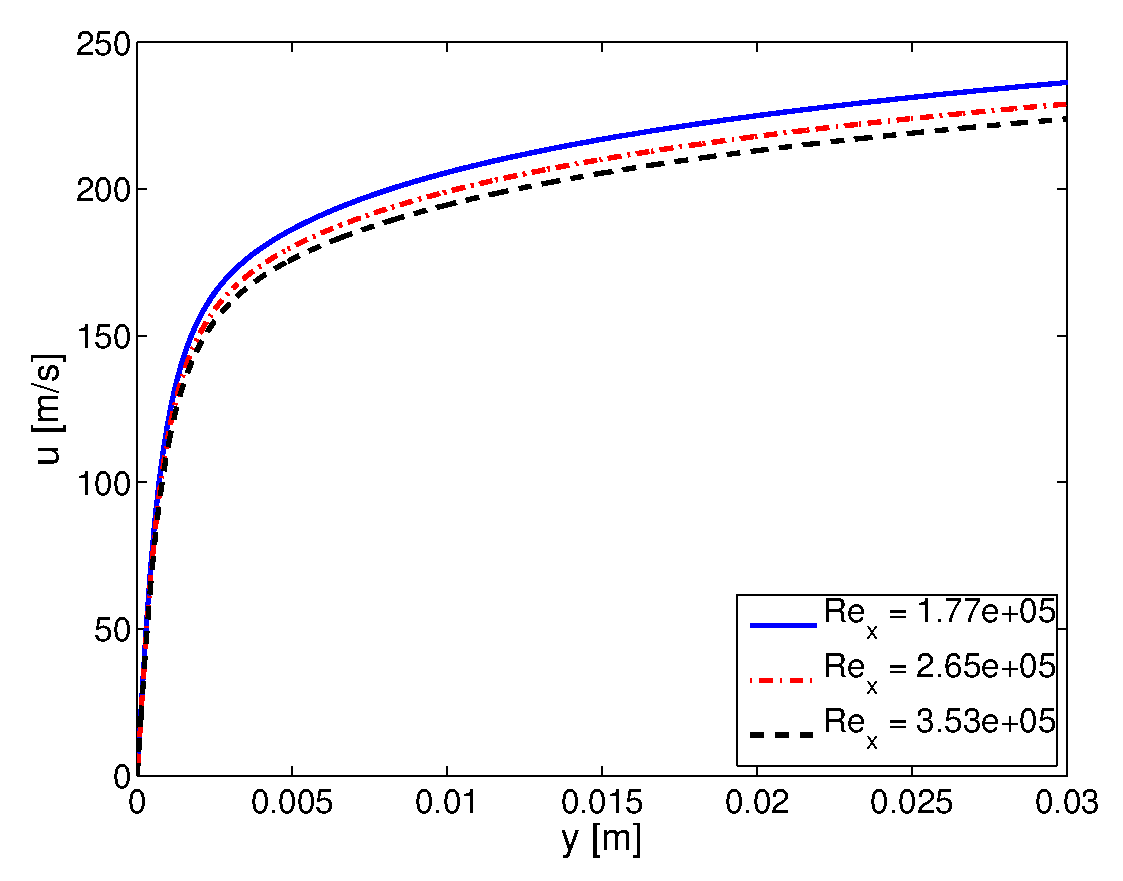
\includegraphics[width=1.15\linewidth]{man_u_dimensional} \\
    \end{center}
    \end{column}

   \begin{column}{5cm}
    \begin{center}
     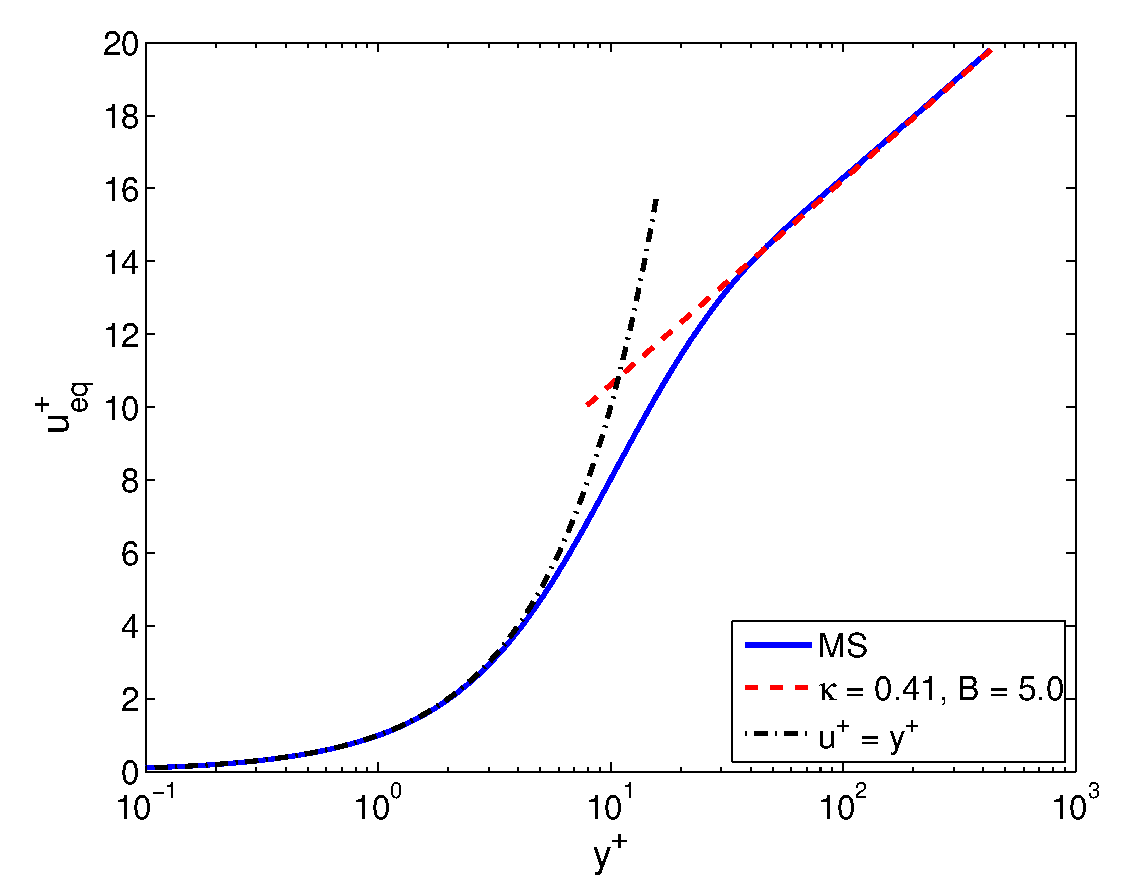
\includegraphics[width=1.15\linewidth]{man_u_nondimensional} \\
    \end{center}
   \end{column}
  \end{columns}
    
 \end{frame}

%===============================================================================
% look ma, pretty
% too much for the young ones, I think
%===============================================================================
% \begin{frame}
%  \frametitle{SA Equation Budgets}

%   \begin{columns}[c]
%     \begin{column}{5cm}

%     \begin{center}
%      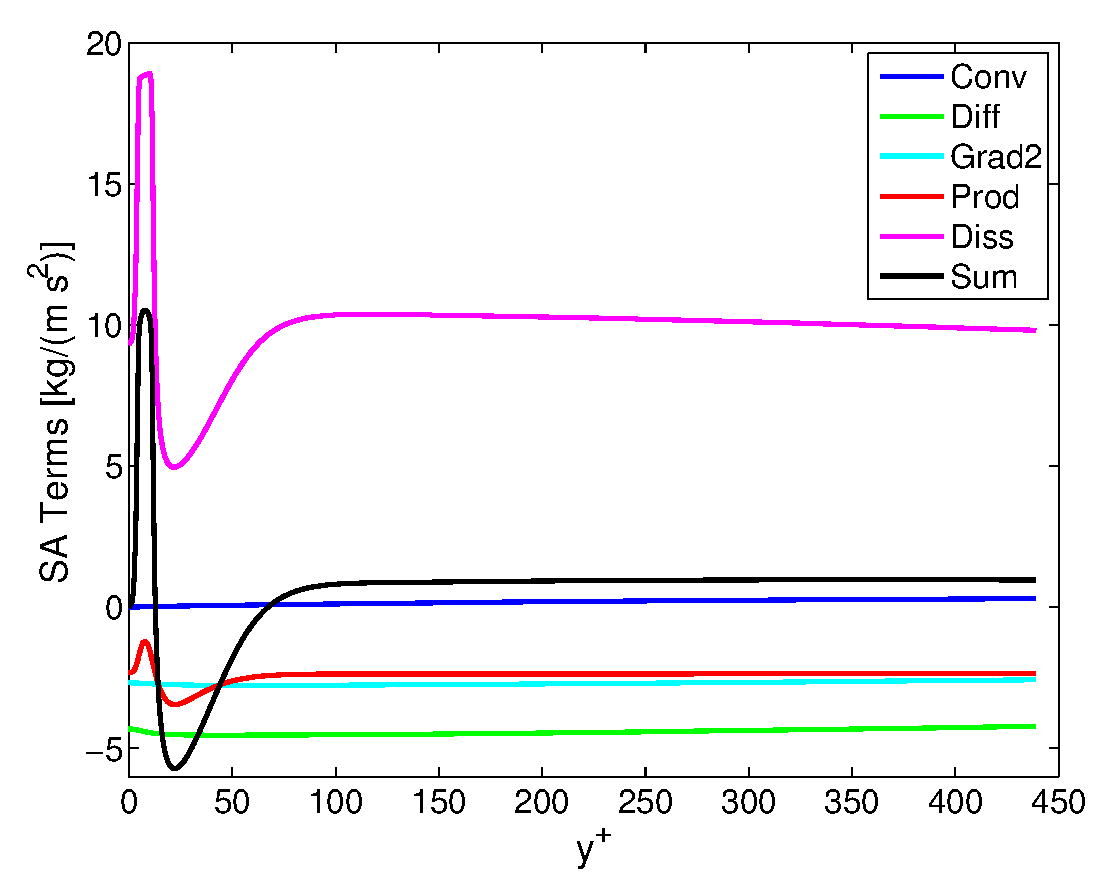
\includegraphics[width=1.15\linewidth]{sa_budget} \\
%     \end{center}

%     \end{column}

%    \begin{column}{5cm}

%     \begin{center}
%      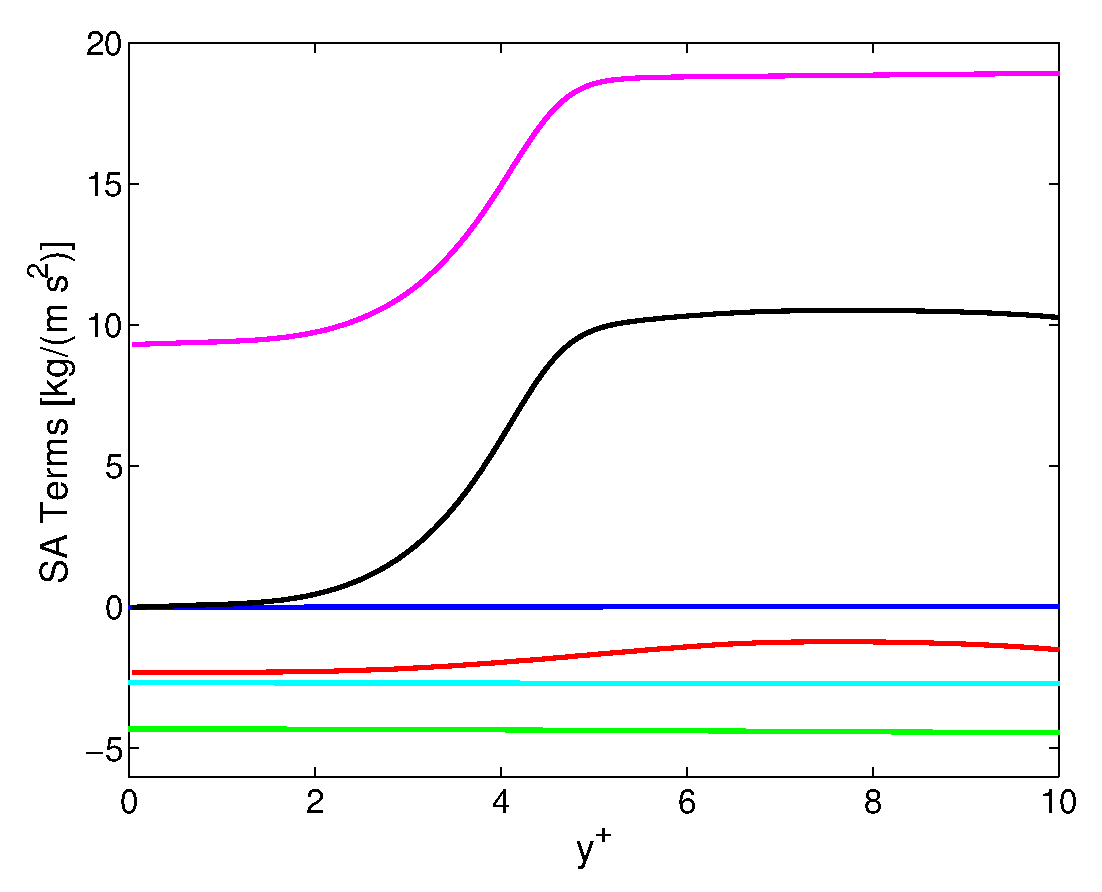
\includegraphics[width=1.15\linewidth]{sa_budget_near_wall} \\
%     \end{center}

%    \end{column}
%   \end{columns}

%  \begin{itemize}
%   \item Inside viscous sublayer, source term is small relative to other
% 	terms
%   \item Production and dissipation terms go to constants at the wall
%   \item Source term is largest in buffer region
%  \end{itemize}

% \end{frame}

%===============================================================================
% look ma, pretty
%===============================================================================
 \begin{frame}
   \frametitle{Convergence Rates: $Re_x$}

  \begin{figure}[th]
   \begin{center}
    \subfigure[$\bar{\rho}$]{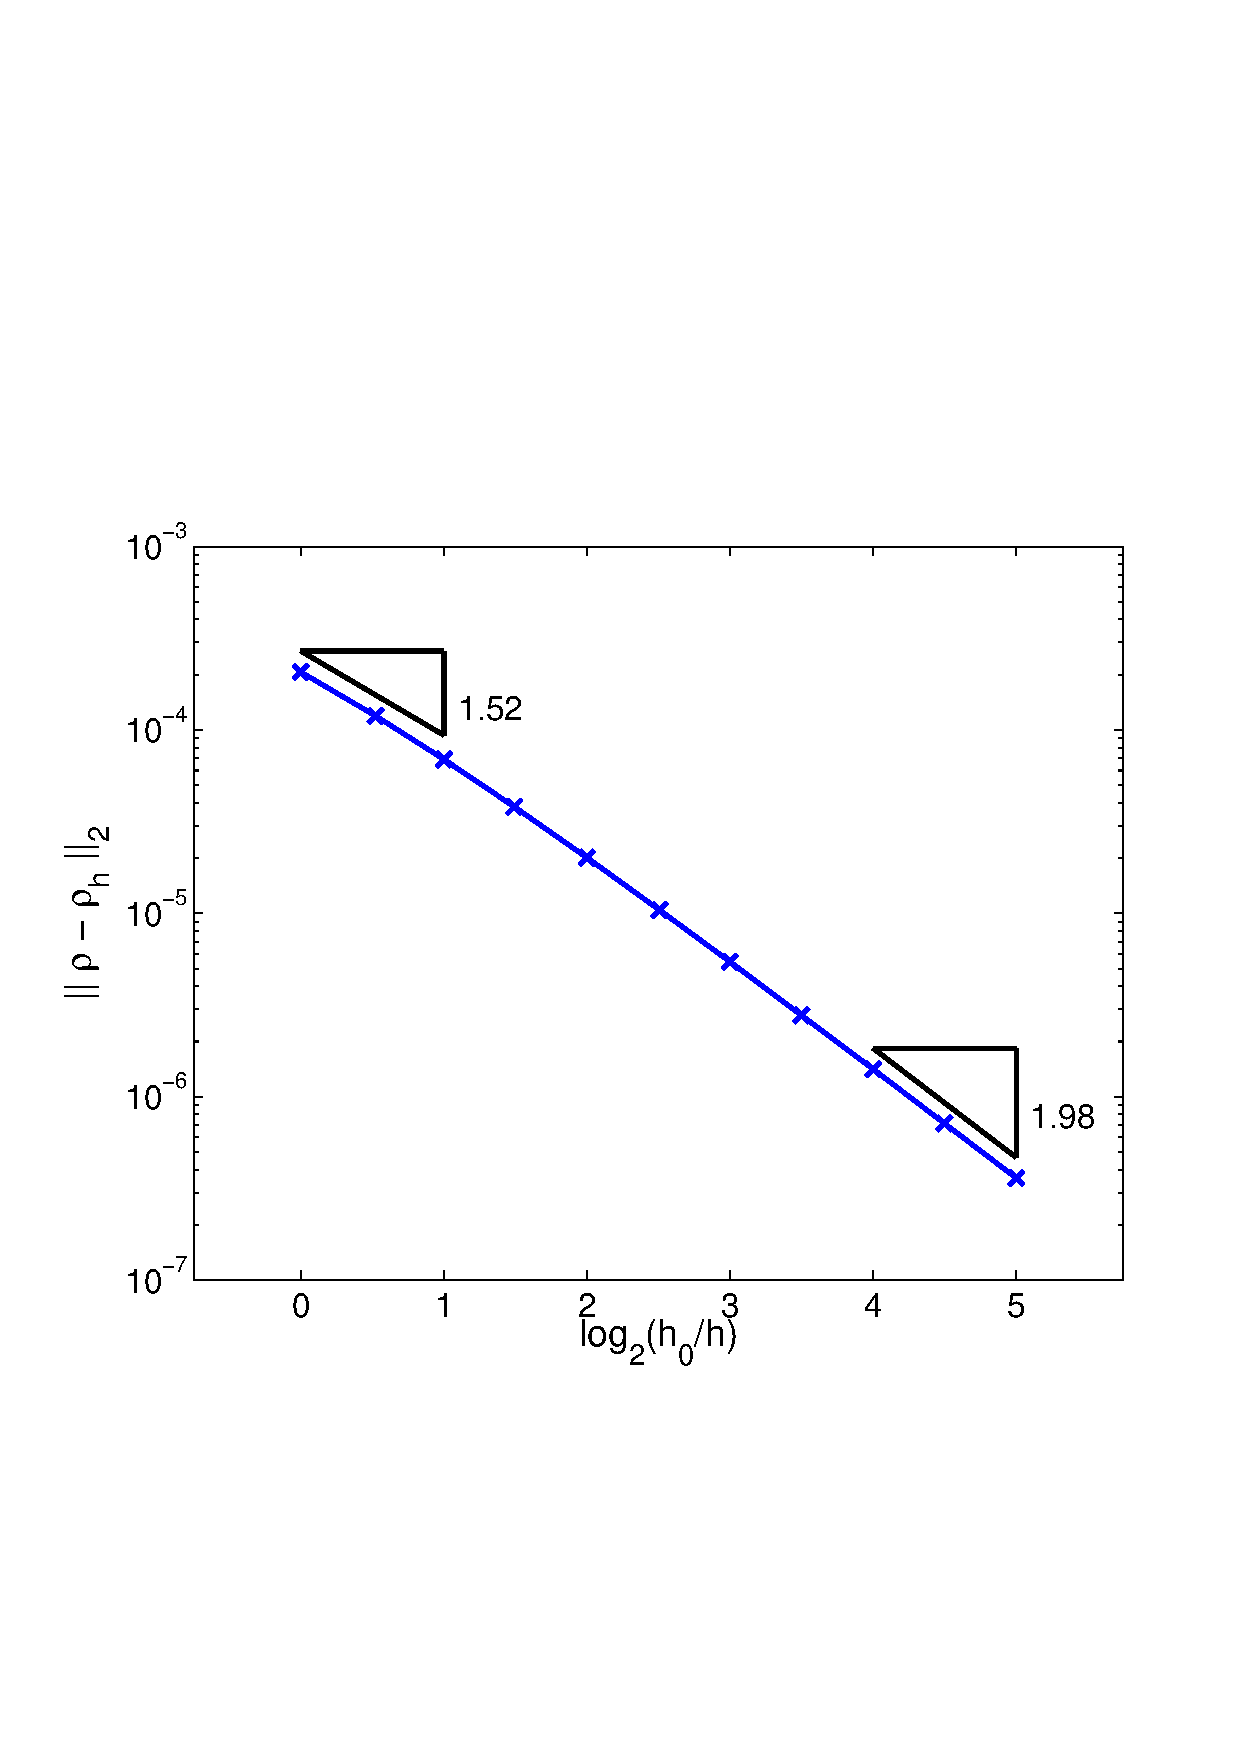
\includegraphics[width=0.33\linewidth]{figs/rho_err_lowRe_wall.pdf}}
    \subfigure[$\bar{\rho} \tilde{u}$]{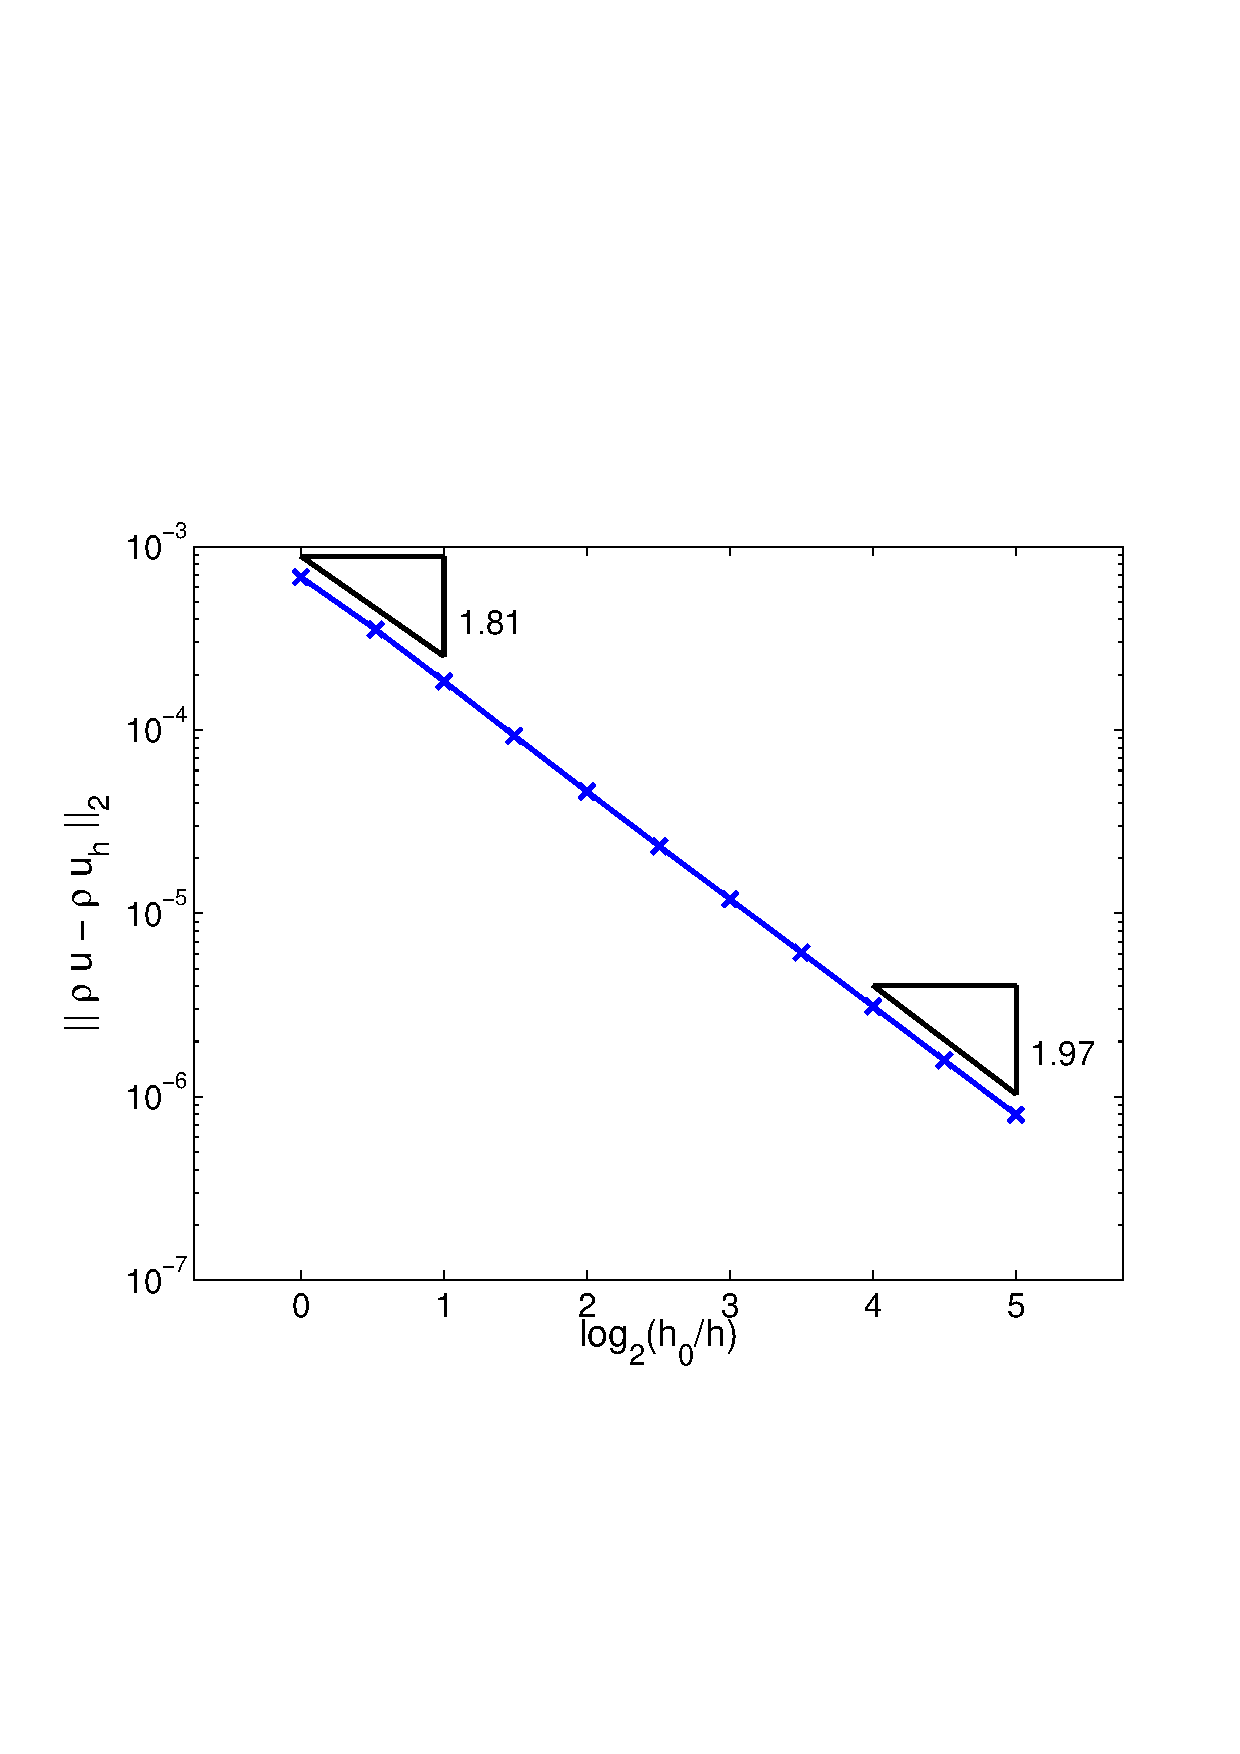
\includegraphics[width=0.33\linewidth]{figs/ru_err_lowRe_wall.pdf}}
    \subfigure[$\bar{\rho} \sa$]{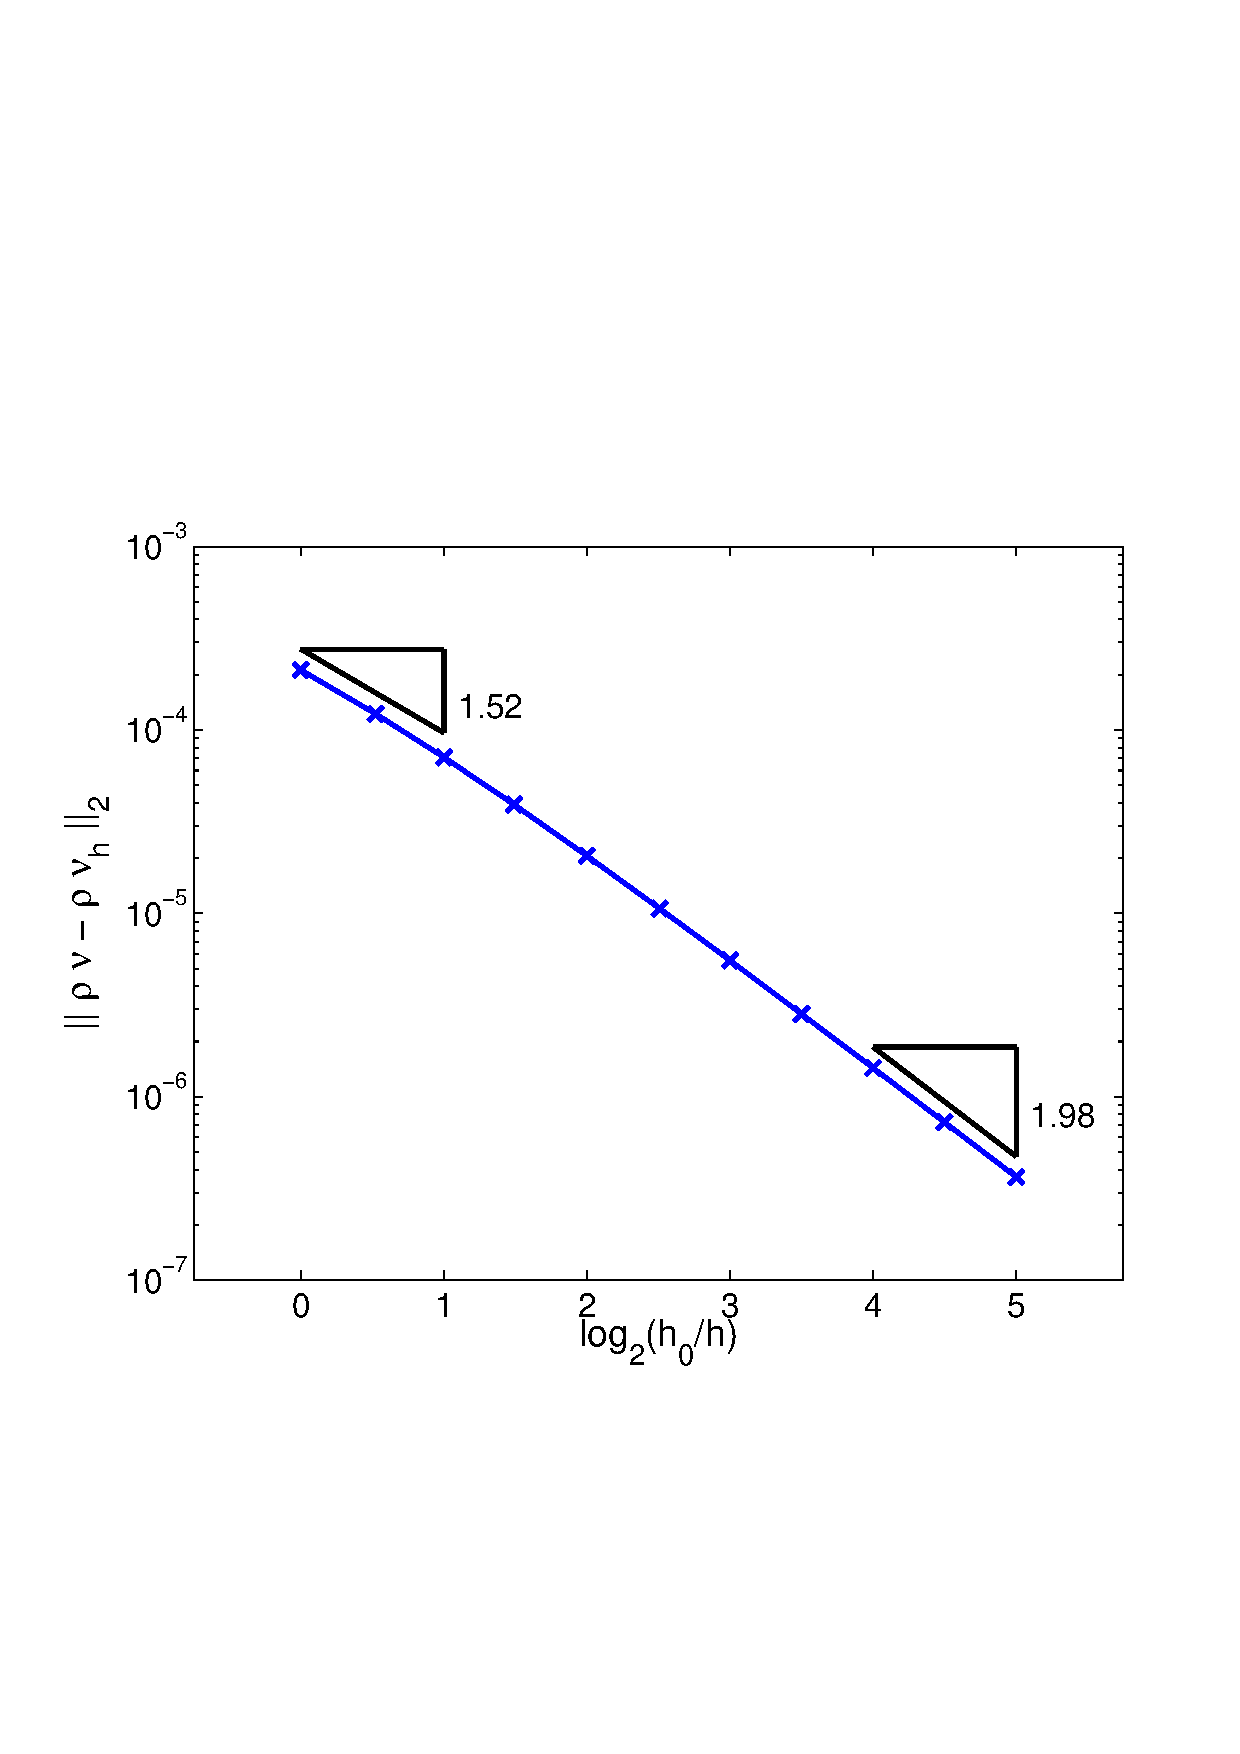
\includegraphics[width=0.33\linewidth]{figs/rnutil_err_lowRe_wall.pdf}}
   \end{center}
   \label{fig:lowRe_free_convergence}
  \end{figure}
 \end{frame}

%===============================================================================
% look ma, pretty
% they wont care about high or low Re
%===============================================================================
 % \begin{frame}
 %   \frametitle{Convergence Rates:  $Re_x = 3.5 * 10^5$}

 %  \begin{figure}[th]
 %   \begin{center}
 %    \subfigure[$\bar{\rho}$]{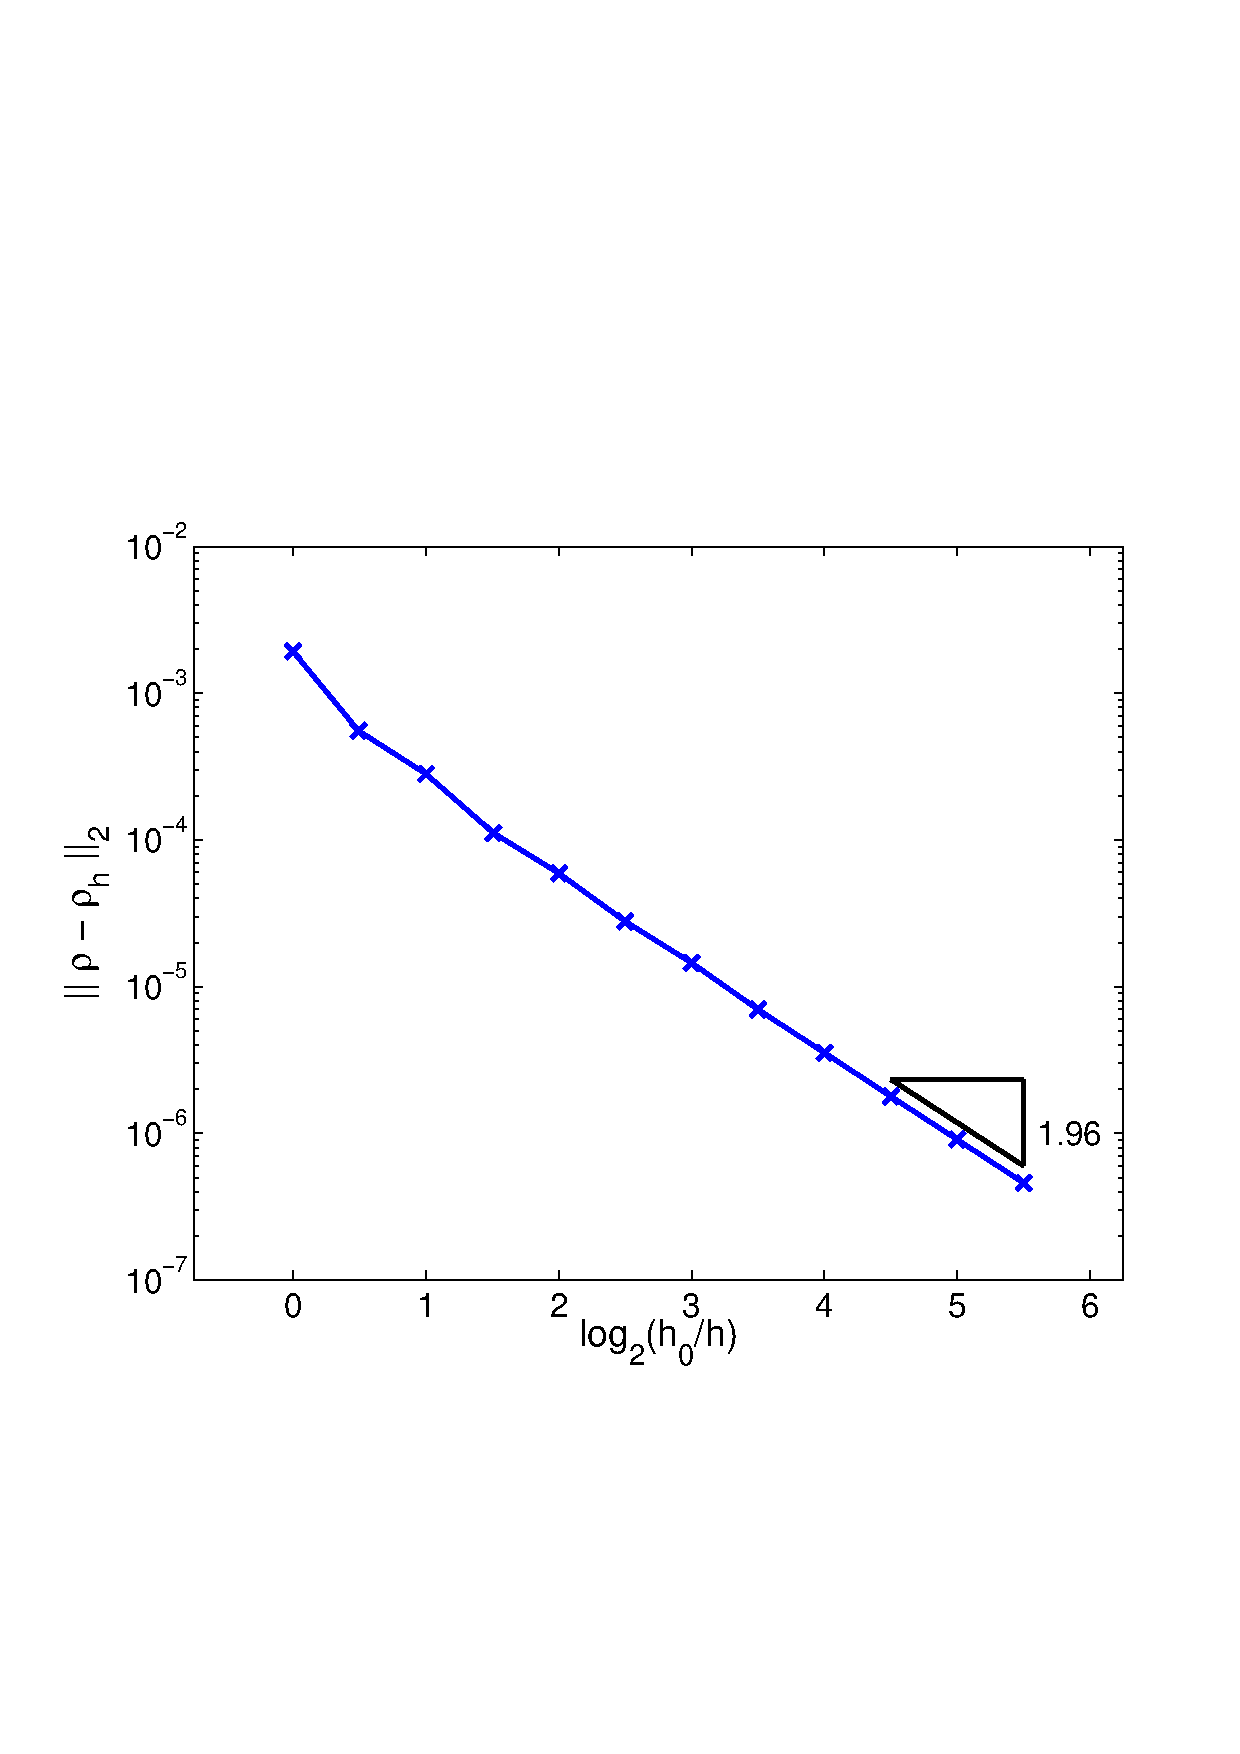
\includegraphics[width=0.33\linewidth]{figs/rho_err_highRe_wall.pdf}}
 %    \subfigure[$\bar{\rho} \tilde{u}$]{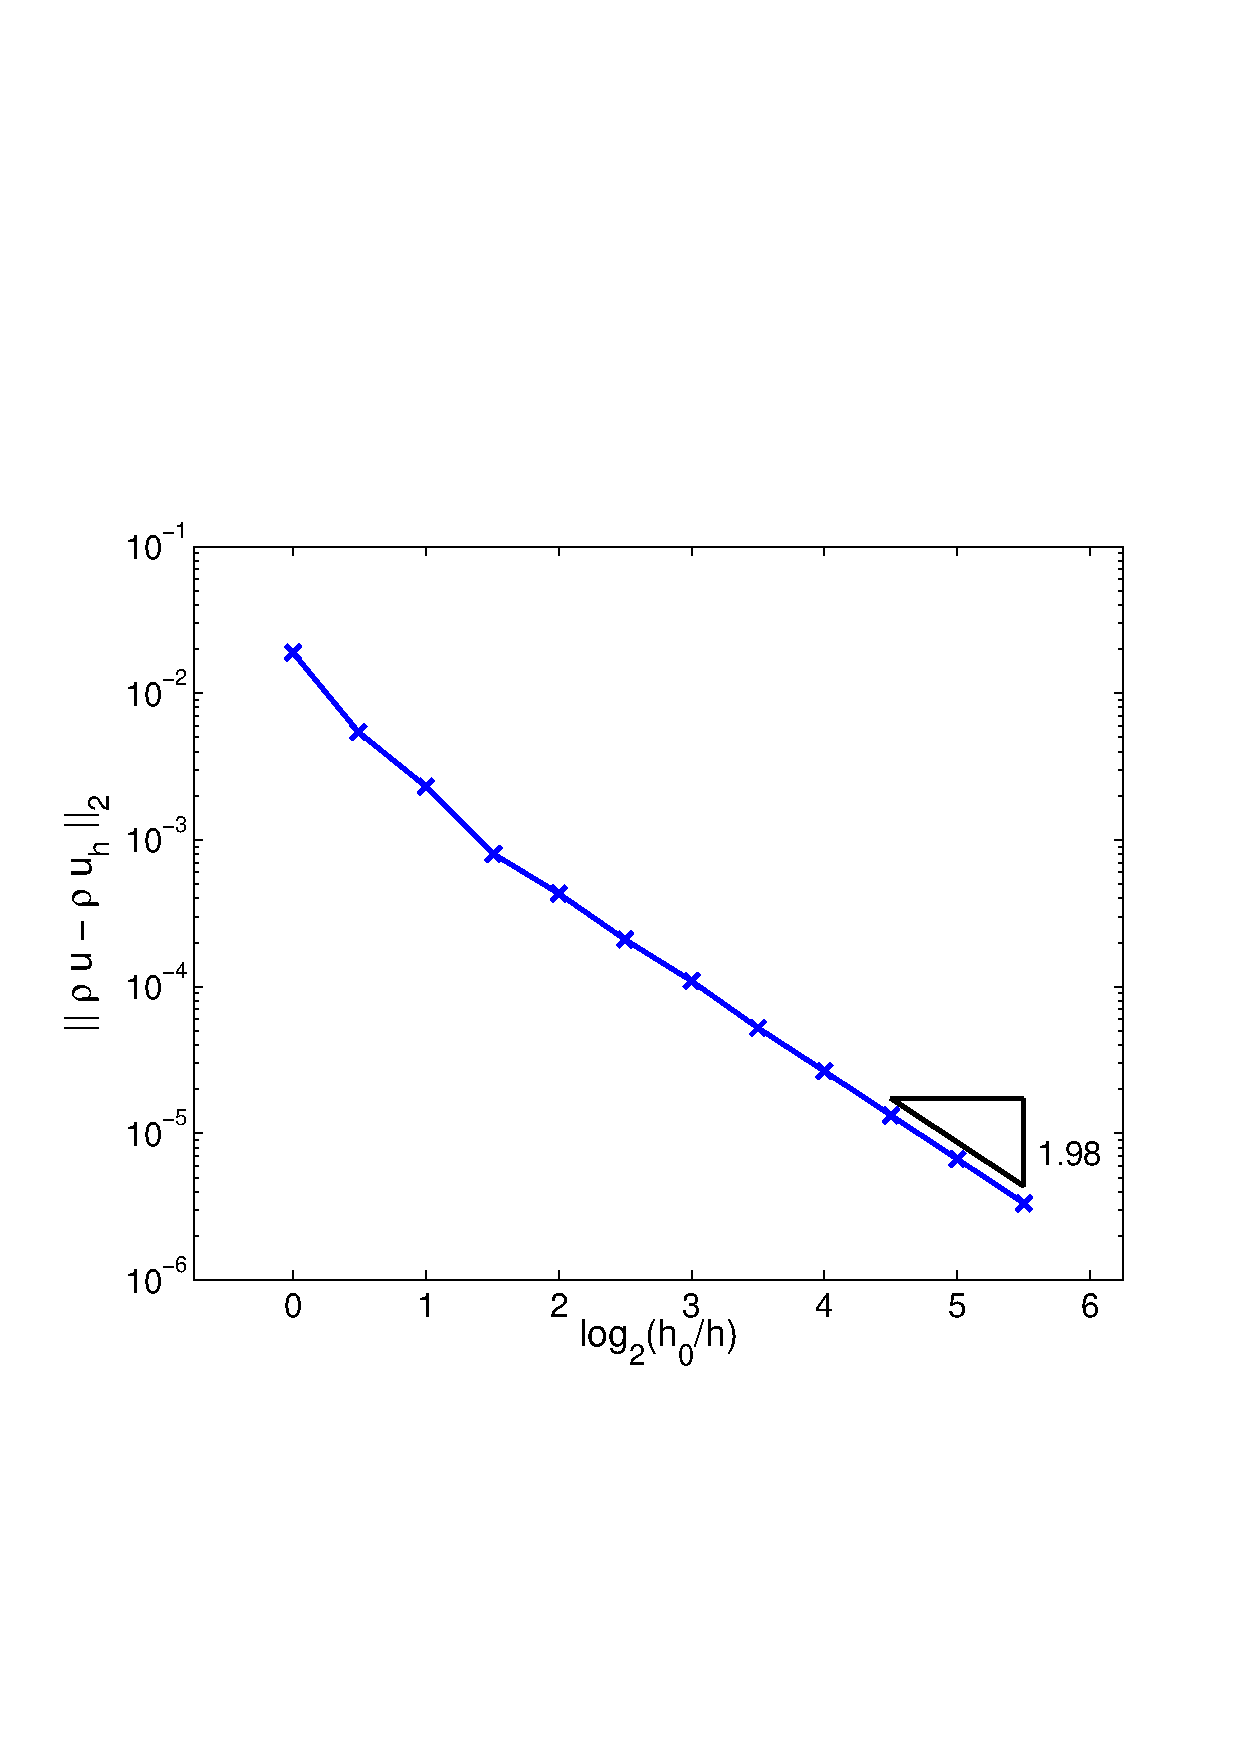
\includegraphics[width=0.33\linewidth]{figs/ru_err_highRe_wall.pdf}}
 %    \subfigure[$\bar{\rho} \sa$]{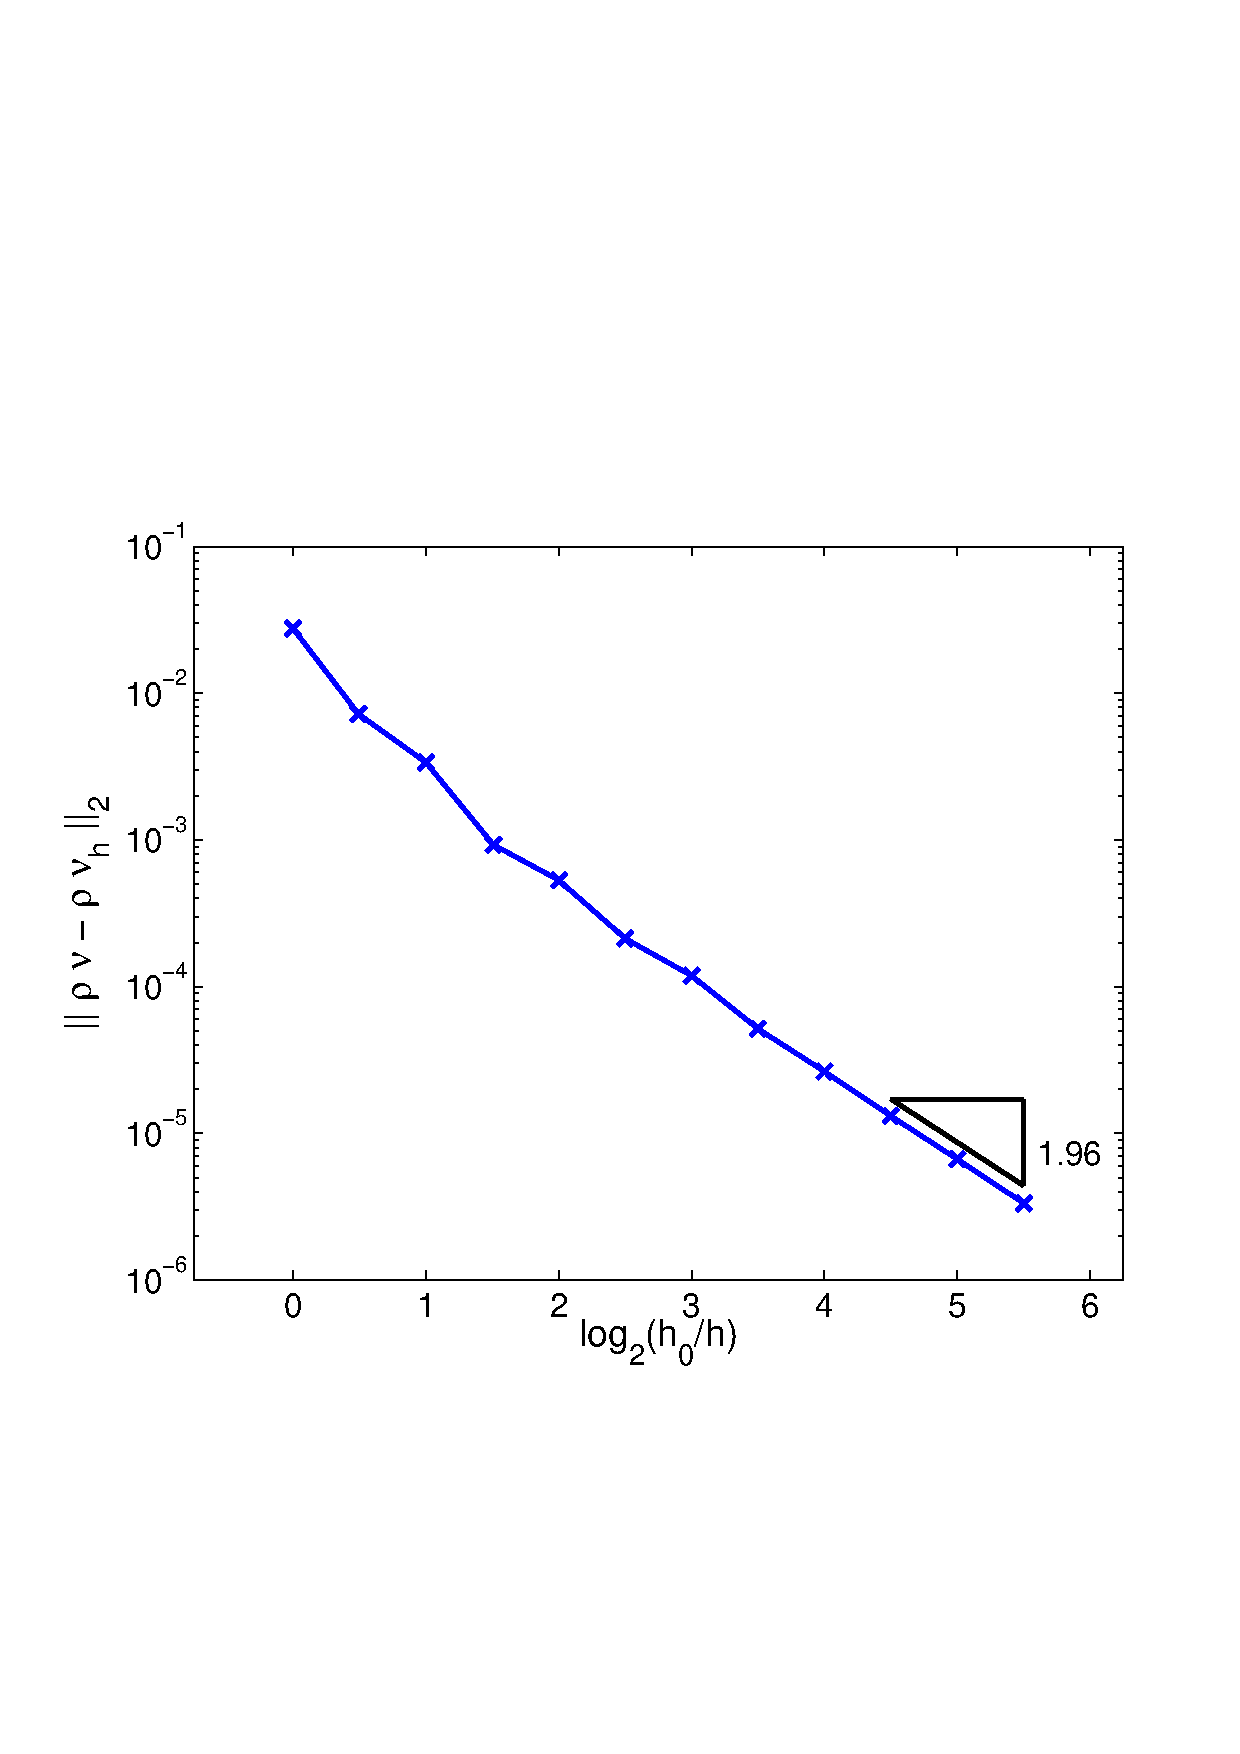
\includegraphics[width=0.33\linewidth]{figs/rnutil_err_highRe_wall.pdf}}
 %   \end{center}
 %   \label{fig:highRe_free_convergence}
 %  \end{figure}
 % \end{frame}

%===============================================================================
% look ma, pretty
%===============================================================================
 \begin{frame}
   \frametitle{Summary}  

  \begin{block}{What we have learned:}  
   \begin{itemize}
    \item Be skeptical of an MS like you would be skeptical of a model
	  \begin{itemize}
	   \item Manufactured Solutions must be verified!
	  \end{itemize}
    \item Exercise each term in the PDE in a similar way to that of a
	  real solution	
    \item {\em More details:} ``Manufactured Solutions for the Favre-Averaged
	  Navier-Stokes Equations with Eddy-Viscosity Turbulence
	  Models''
	  \begin{itemize}
	   \item AIAA 50th Aerospace Sciences Meeting
	  \end{itemize}
	 
   \end{itemize}
  \end{block}

  \begin{block}{Why is this not more commonly done?}  
   \begin{itemize}
    \item Manufactured Solution generation is a time consuming process
	  \begin{itemize}
	   \item Rule of 10\%
	  \end{itemize}
    \item Domain expert input needed to generate manufactured solutions!
   \end{itemize}
  \end{block}
 \end{frame}

%===============================================================================
% maple
%===============================================================================
\begin{frame}
  \frametitle{Manufactured Analytical Solutions Abstractions Library}

  \textcolor{orange}{Goal}: Provide a repository and standardized interface for MMS usage

  \begin{block}{High Priority:}  
    \begin{itemize}
    \item Extreme fidelity to generated MMS
    \item Portability
    \item Traceability
    \item Extensible
    \end{itemize}
  \end{block}

  \begin{block}{Low Priority:}  
    \begin{itemize}
    \item Speed/Performance
    \end{itemize}
  \end{block}

\end{frame}

%===============================================================================
% verifying masa
%===============================================================================
\begin{frame}[fragile]
  \frametitle{Verifying the ``Verifier''}  
  Precision is not negotiable.
  \begin{columns}[c]
    \begin{column}{7cm}

      % kill?
      %\begin{block}{\small Maple Testing}
      %  \begin{itemize}
      %    \item \small factored source terms subtracted from unsimplified
      %  \end{itemize}
      %\end{block}

      % add mention of new flags on 

      \begin{block}{\small MASA Testing}
        \begin{itemize}
        \item \small Error target $<$ 1e-15
          \begin{itemize}
            \small
            \item Absolute error on local machines
            \item Relative error (other)
            \item On all supported compiler sets
          \end{itemize}
        \item \small -O0 not sufficient
          \begin{itemize}
            \small
            \item -fp-model precise (Intel)
            \item -fno-unsafe-math-optimizations (GNU)
            \item -Kieee -Mnofpapprox (PGI)
          \end{itemize}
        \item \small ``make check''
          \begin{itemize}
          \item \small Run by Buildbot every two hours
          \end{itemize}
          \normalsize
        \end{itemize}        
      \end{block}
    \end{column}
    \begin{column}{4.2cm}
      {\tiny
\begin{verbatim}
[nick@magus trunk]$ make check
-----------------------------------------
Initializing MASA Tests
-----------------------------------------
PASS: init.sh
PASS: misc
PASS: fail_cond
PASS: catch_exception
PASS: register
PASS: poly
PASS: uninit
PASS: vec
PASS: purge
PASS: heat_const_steady
PASS: euler1d

\end{verbatim}
$\vdots$\hspace*{6em}$\vdots$
\begin{verbatim}

-----------------------------------------
Finalizing MASA Tests
-----------------------------------------
===================
All 65 tests passed
===================
\end{verbatim}
      }
    \end{column}
  \end{columns}

\end{frame}

%===============================================================================
% masa developments parameters
%===============================================================================
\begin{frame}
  \frametitle{Portability}  

  \begin{columns}[c]
    \begin{column}{5cm}
      \begin{block}{Software Environment}  
        \begin{itemize}
          \small
        \item Built with: Autotools, C++
        \item Supports Intel, GNU, Portland Group compilers
        \item C/C++ interfaces
        \item Fortran interfaces provided through \textcolor{orange}{iso\_c\_bindings}
          \begin{itemize}
          \item \tiny Fortran 2003 Standard
          \end{itemize}
        \item Python interfaces generated with \textcolor{blue}{SWIG}
        \end{itemize}          
      \end{block}
    \end{column}

    \begin{column}{5cm}
      \begin{block}{Testing}  
        \begin{itemize}
        \item \small GIT: version control
        \item \small Buildbot: automated testing
        \item \small GCOV: line coverage
          \begin{itemize}
          \item \small 15,826 lines of code
          \item \small 13,195 lines of testing
          \item \small 98\%+ line coverage
          \end{itemize}          
        \end{itemize}          
      \end{block}

     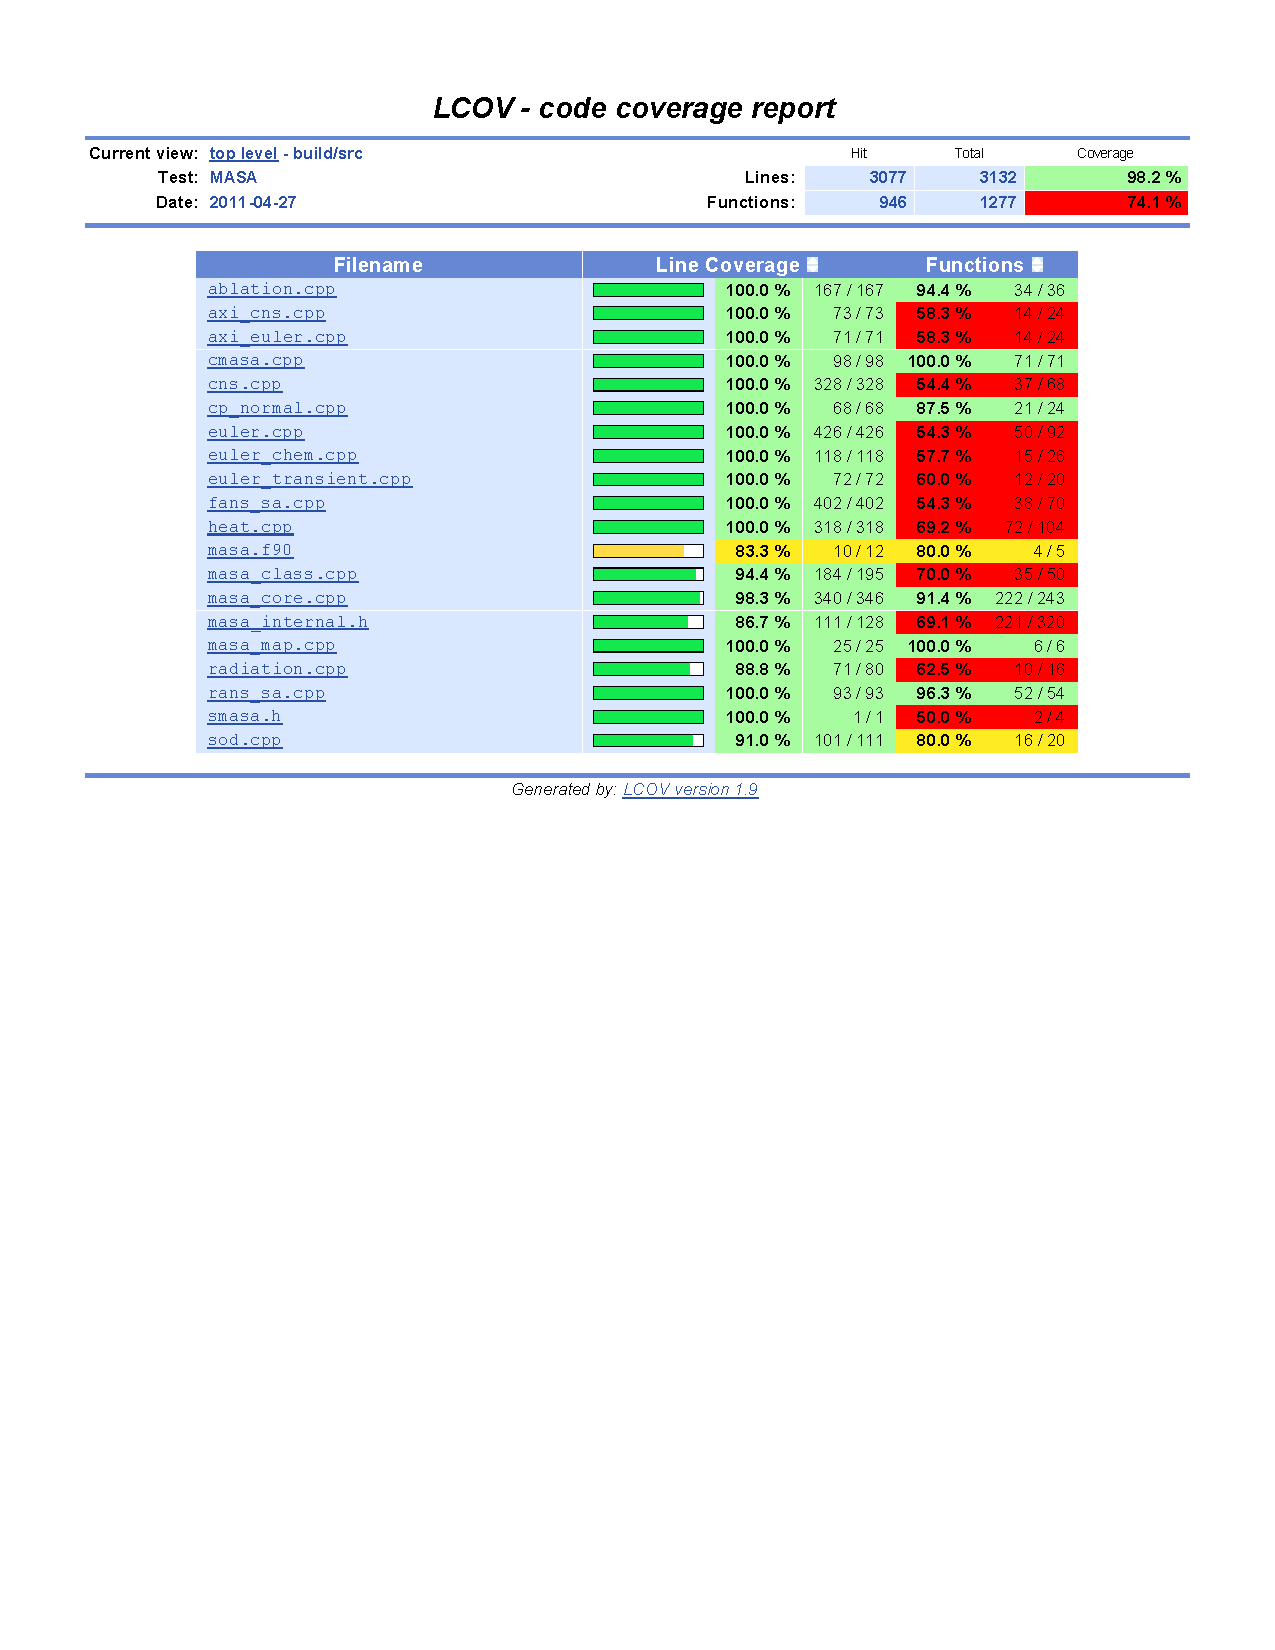
\includegraphics[scale=0.25]{masa-gcov}
  
    \end{column}
  \end{columns}

\end{frame}

%===============================================================================
% doxygen
%===============================================================================

\begin{frame}
  \frametitle{Traceability}
  Doxygen provides code and model documentation
  \begin{columns}[c]

    \begin{column}{6cm}
      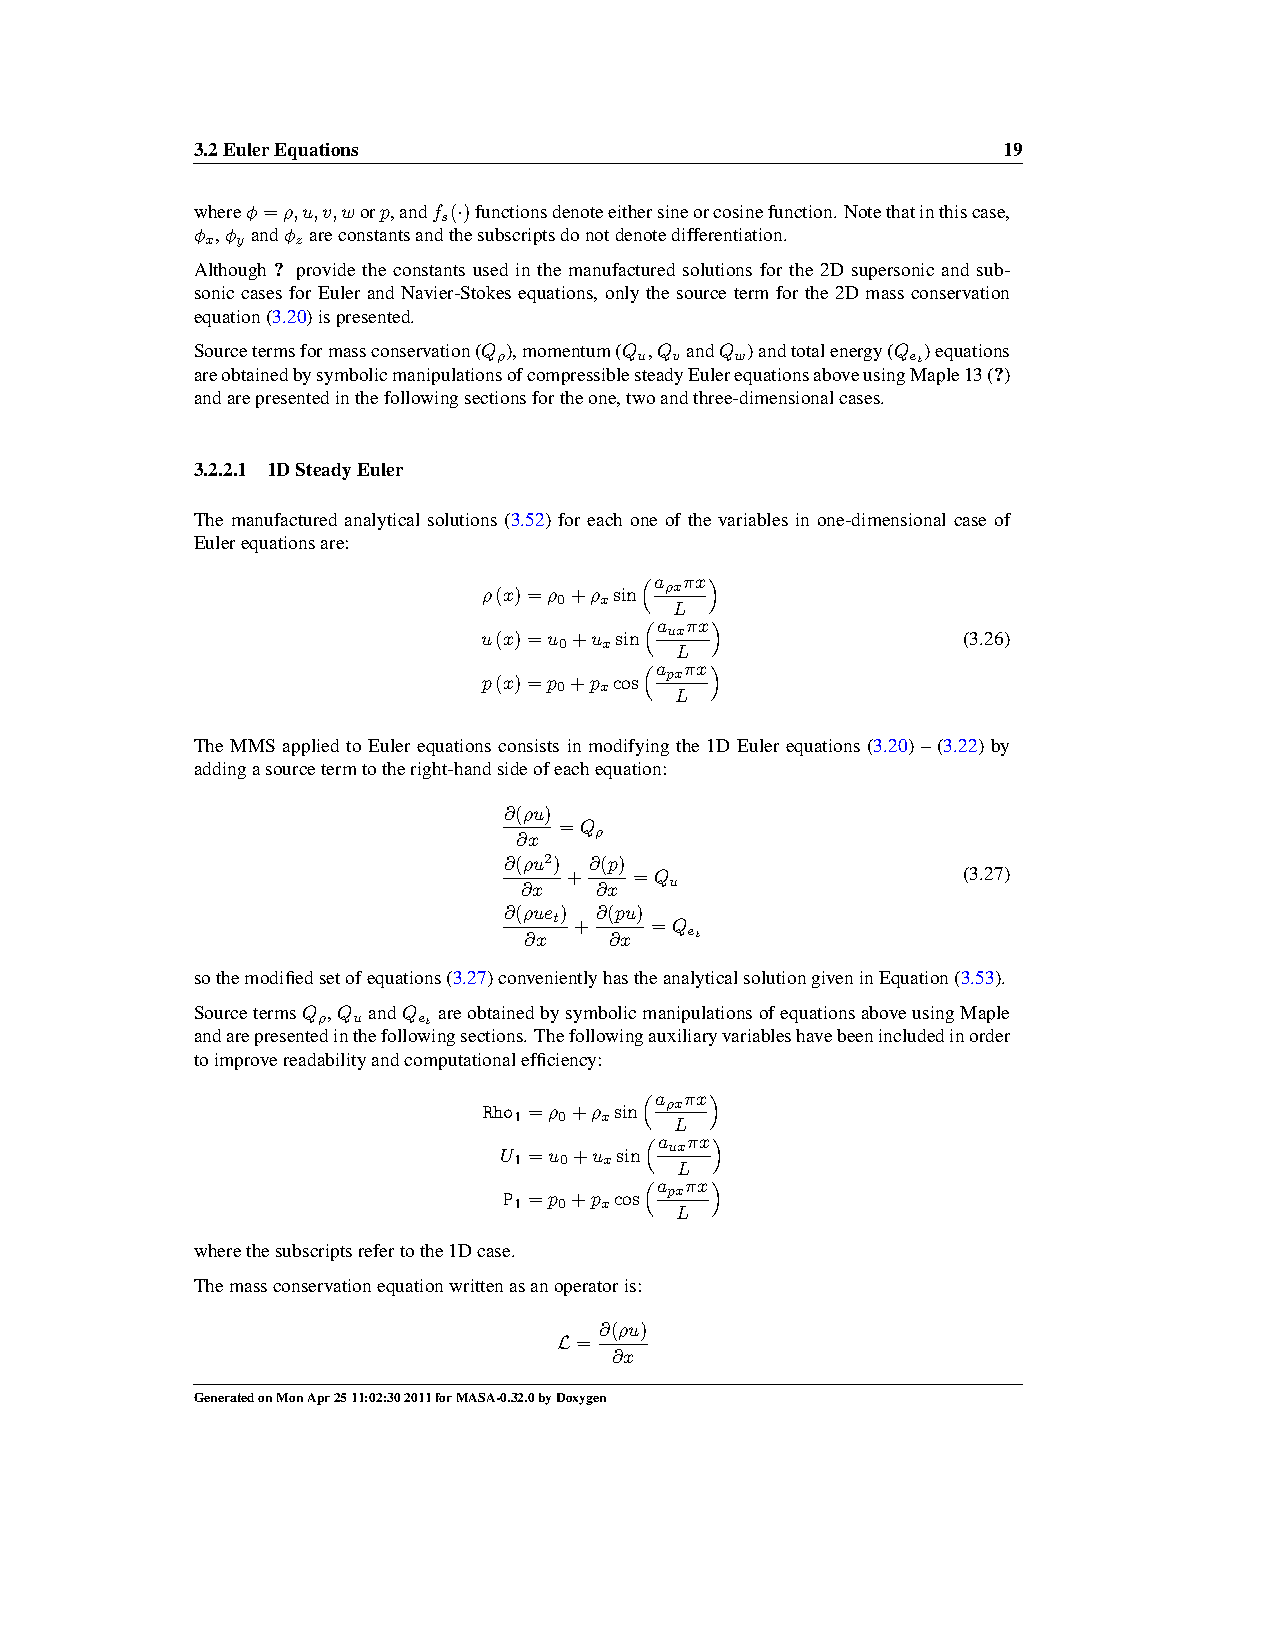
\includegraphics[scale=.31]{euler}   \\
    \end{column}

    \begin{column}{12cm}
      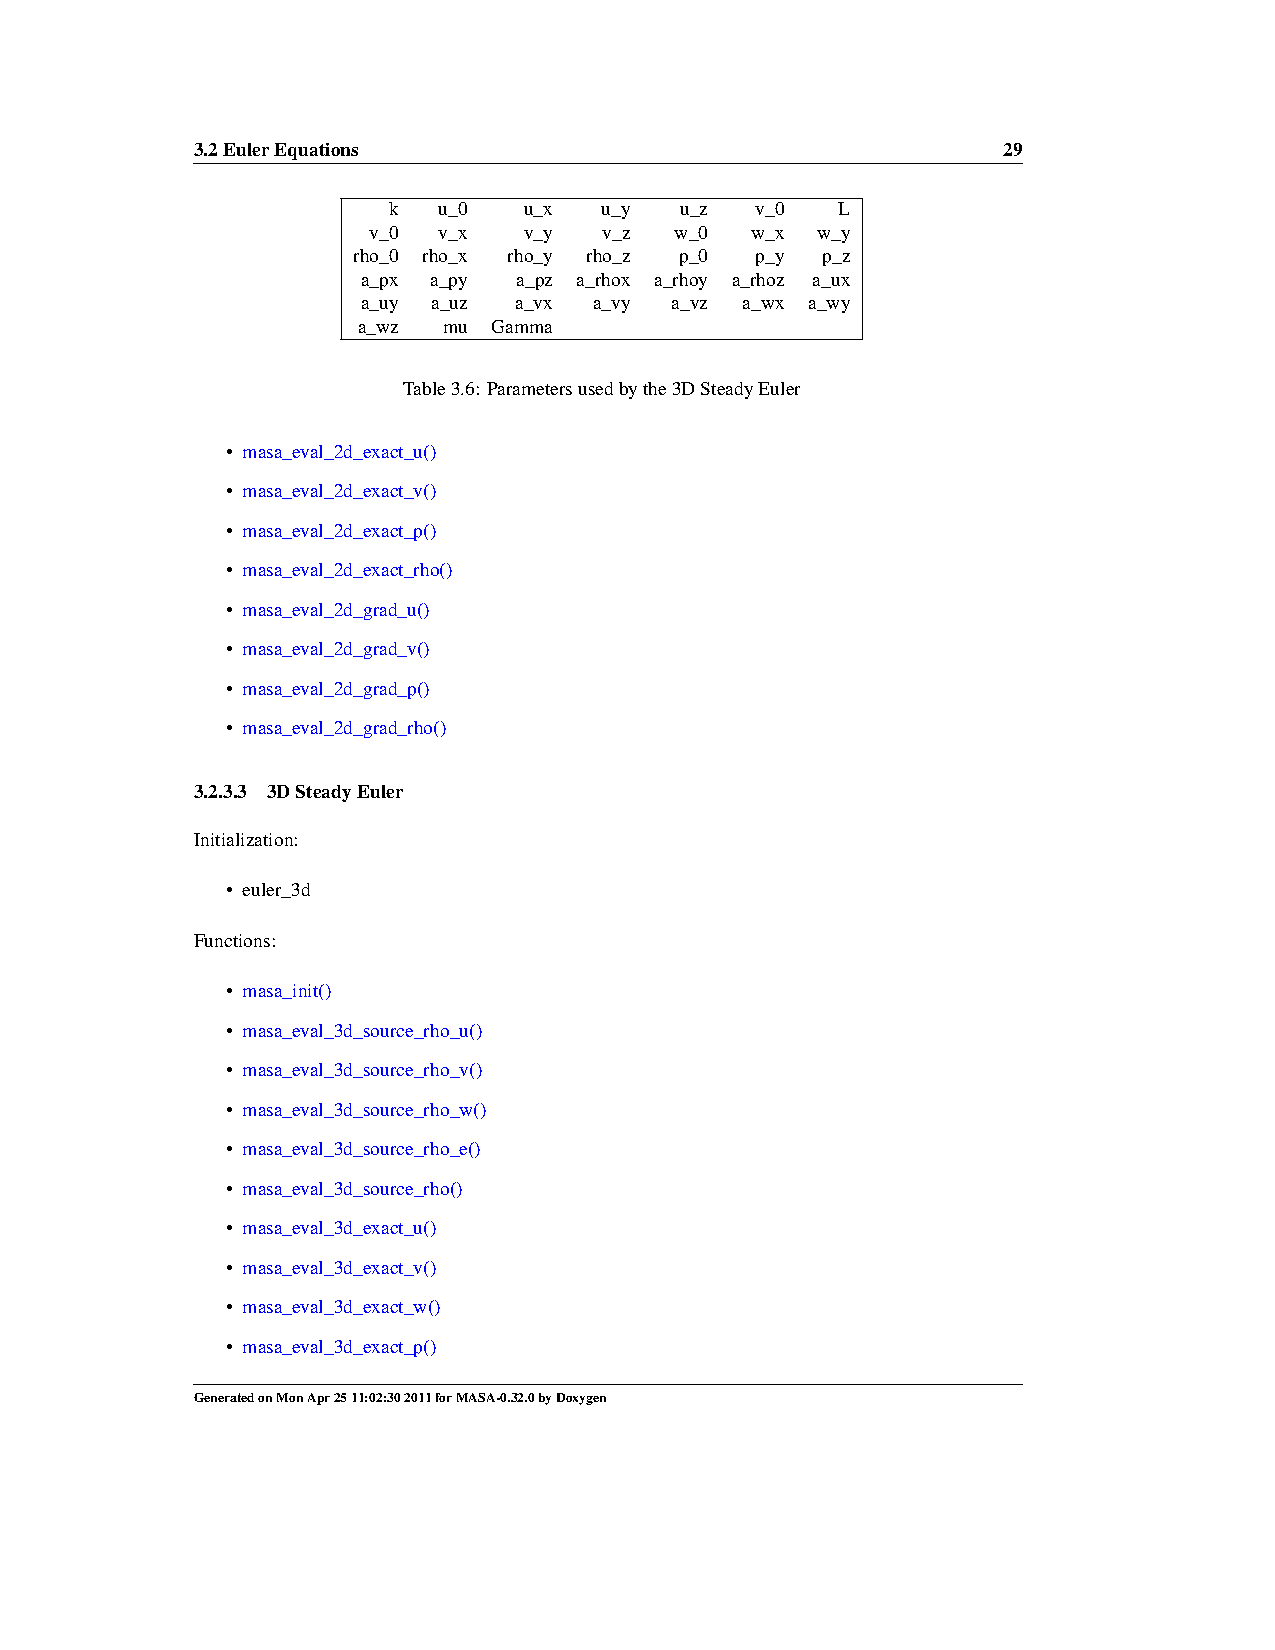
\includegraphics[scale=.31]{euler_api} \\
    \end{column}

  \end{columns}    

\end{frame}

%===============================================================================
% talk about how the solutions ``look'', physically
%===============================================================================
\begin{frame}
  \frametitle{Providing Reasonable Defaults}

  \begin{block}{Requirements:}
  \begin{itemize}
    \item Sufficient algebraic complexity to exercise all terms
    \item Physically consistent
      \begin{itemize}
        \item e.g. solutions should not return negative densities, temperatures, etc.
      \end{itemize}      
  \end{itemize}
  \end{block}

  \begin{center}
    \includegraphics[scale=.3]{pressure}\\
  \end{center}

\end{frame}

%===============================================================================
% NEW SLIDE: boundary conditions
%===============================================================================
%% \begin{frame}
%% \frametitle{Boundary Condition Verification}

%% \begin{block}{Recommendation: Boundary Condition Verification Using MMS}
%% \begin{itemize}
%%   \item All codes have been verified using Dirchlet boundary conditions.    
%%   \item Accomplished by evaluating analytical terms on the domain edge
%% \end{itemize}
%% \end{block}

%% \begin{block}{Additional Boundary Conditions:}
%%   \begin{itemize}
%%   \item MASA now provides gradients of all manufactured analytical solutions

%%     \begin{itemize}
%%       \item enables Neumann boundary condition verification
%%     \end{itemize}
%%   \item Ablation MMS required integrating the manufactured solutions over the boundary
%%   \end{itemize}
%% \end{block}

%% \end{frame}

%===============================================================================
% masa in pecos codes
%===============================================================================
%% \begin{frame}
%%   \frametitle{MASA + PECOS Codebase Integration}
%%   \begin{columns}[c]
%%     \begin{column}{7cm}
%%       \begin{table}
%%         \centering
%%         \begin{tabular}{|c c|}
%%           \hline 
%%           Codebase     & Solution \\
%%           \hline
%%           WENO         & Euler                \\
%%           Thermocouple & Heat                 \\
%%           Radiation    & Integrated intensity \\
%%           compDNS      & Navier-Stokes        \\
%%           QUESO        & Conjugate prior      \\ 
%%           \hline
%%           FIN-S        & Navier-Stokes      \\
%%                        & Euler              \\
%%                        & Euler + chemistry  \\
%%                        & N-S + ablation     \\
%%           \hline 
%%           \textcolor{orange}{Suzerain} & Navier-Stokes \\
%%           \textcolor{orange}{Chemay}   & chemistry     \\
%%           \hline 
%%         \end{tabular}
%%       \end{table}
%%     \end{column}

%%     \begin{column}{4cm}
%%       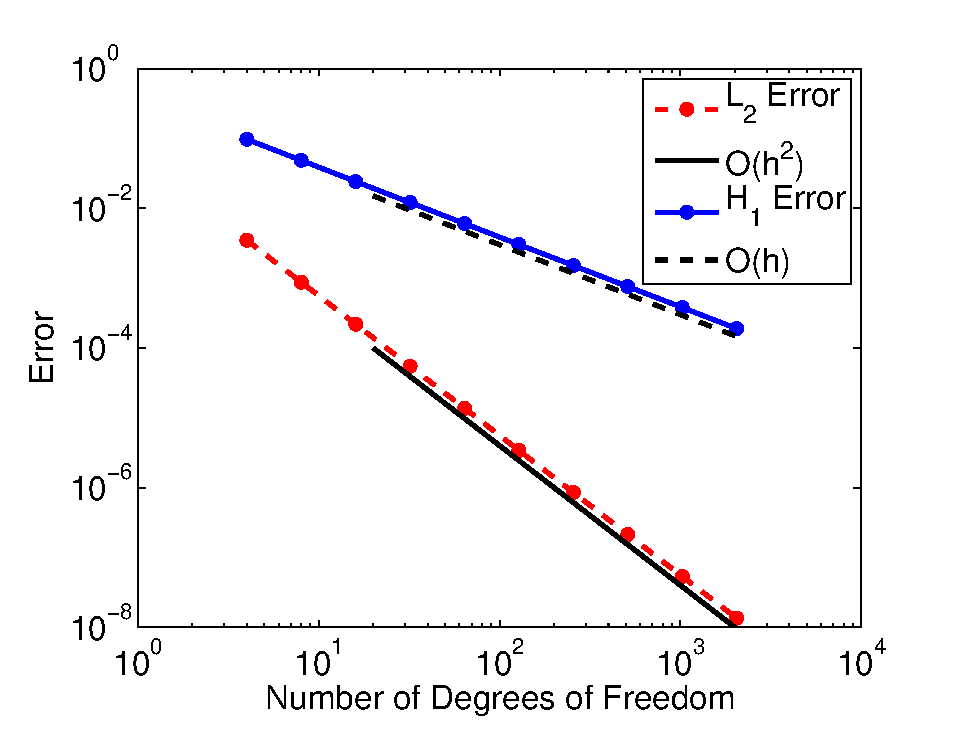
\includegraphics[width=1.1\linewidth]{thermo} \\
%%       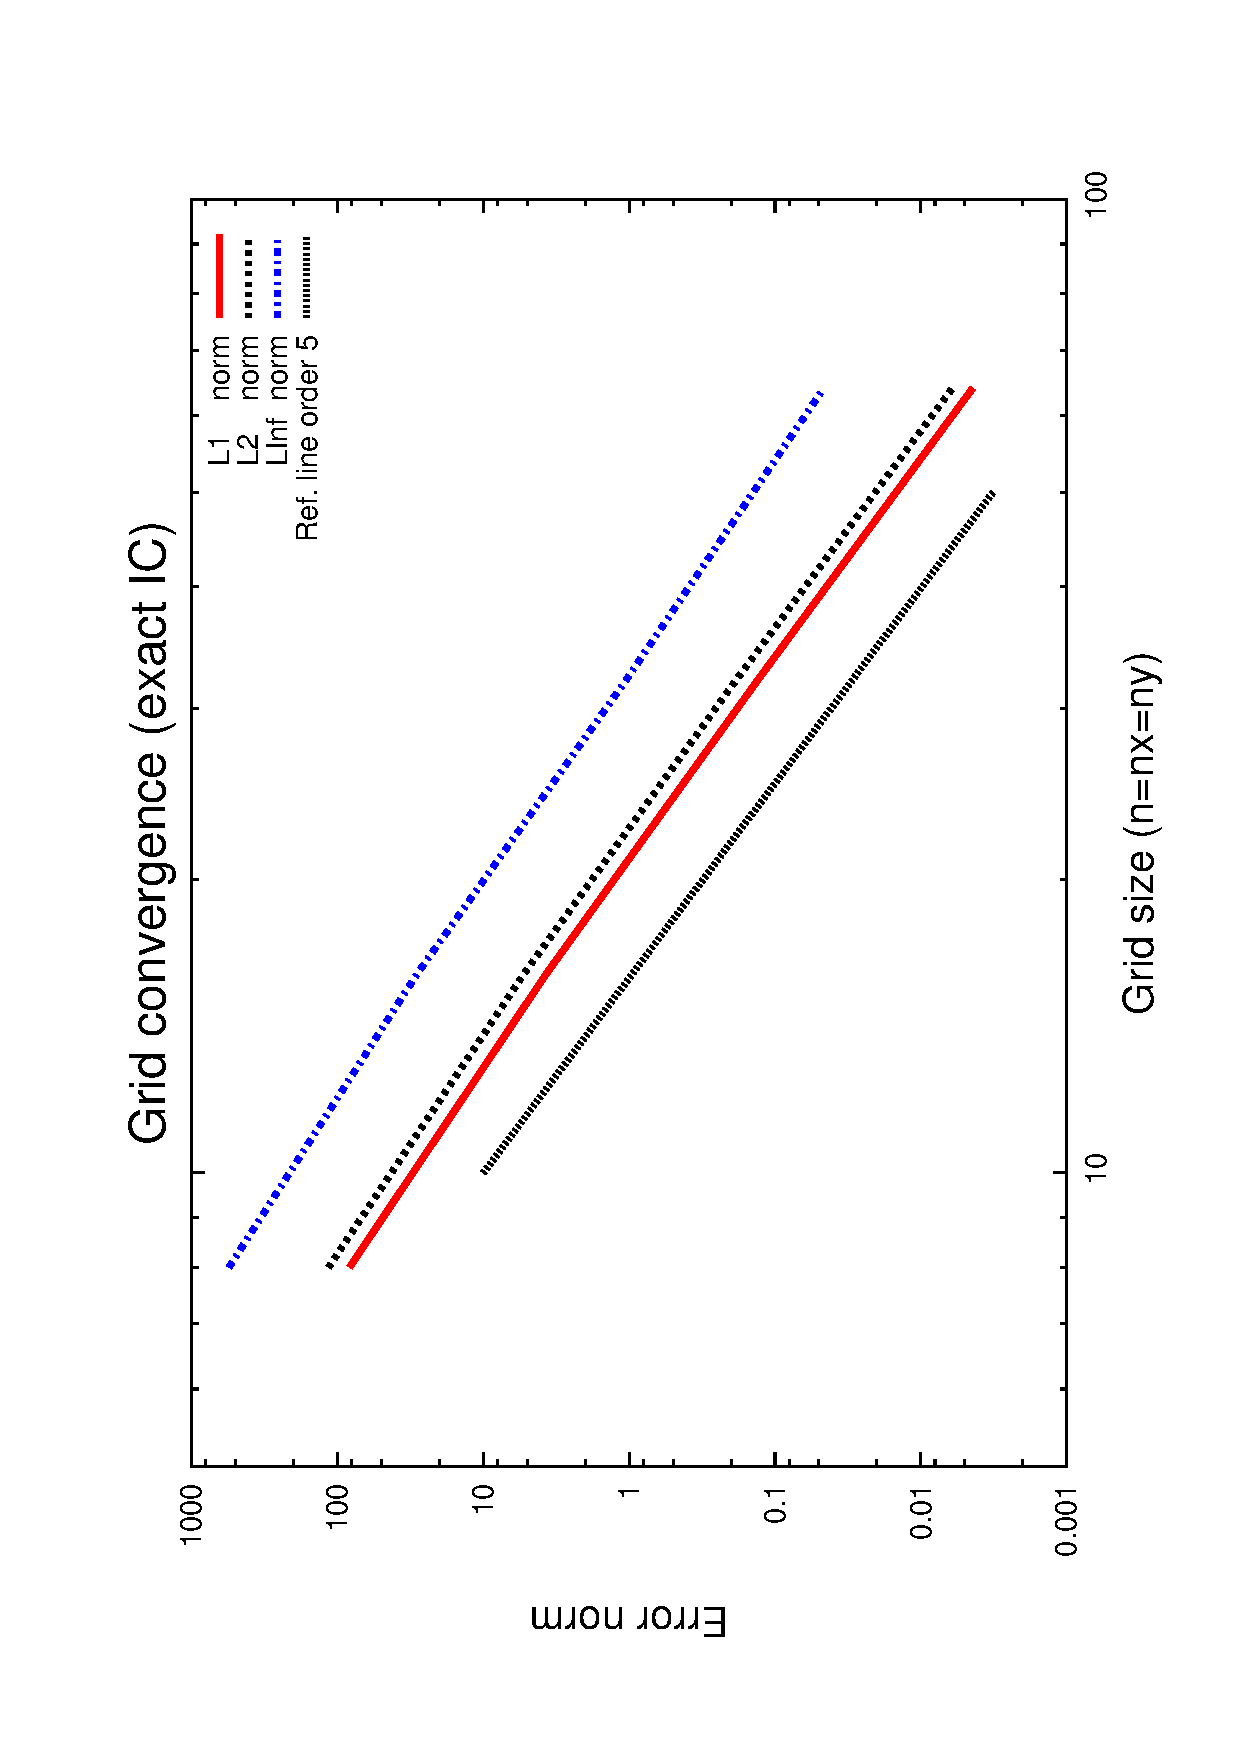
\includegraphics[width=1.1\linewidth]{compdns} \\ 
%%     \end{column}

%%   \end{columns}
%% \end{frame}

%===============================================================================
% NEW SLIDE: table of available solutions
%===============================================================================
\begin{frame}
  \frametitle{Available Solutions in MASA 0.44.0}

  \begin{table}
    \centering
    \begin{tabular}{c c c c}
      \hline
      Equations & Dimensions & Time \\
      \hline \vspace{-8pt} \\
      Euler                      & 1,2,3, axi & Transient, Steady \\
      Non linear heat conduction & 1,2,3 & Transient, Steady \\
      Navier-Stokes              & 1,2,3, axi & Transient, Steady \\
      N-S + Sutherland           &     3 & Transient, Steady \\
      N-S + ablation             &     1 & Transient, Steady \\
      Burgers                    &     2 & Transient, Steady \\ 
      Sod Shock Tube             &     1 & Transient \\
      Euler + chemistry          &     1 & Steady    \\
      RANS: Spalart-Allmaras     &     1 & Steady \\
      FANS: SA                   &     2 & Steady \\
      FANS: SA + wall            &     2 & Steady \\
      Radiation                  &     1 & Steady \\ 
      SMASA: Gaussian            &     1 & Steady \\ 
      \hline
    \end{tabular}
  \end{table}
\end{frame}


%===============================================================================
% application linkage
%===============================================================================
\begin{frame}
  \frametitle{General Verification Approach Using MMS and MASA}
  \begin{center}
    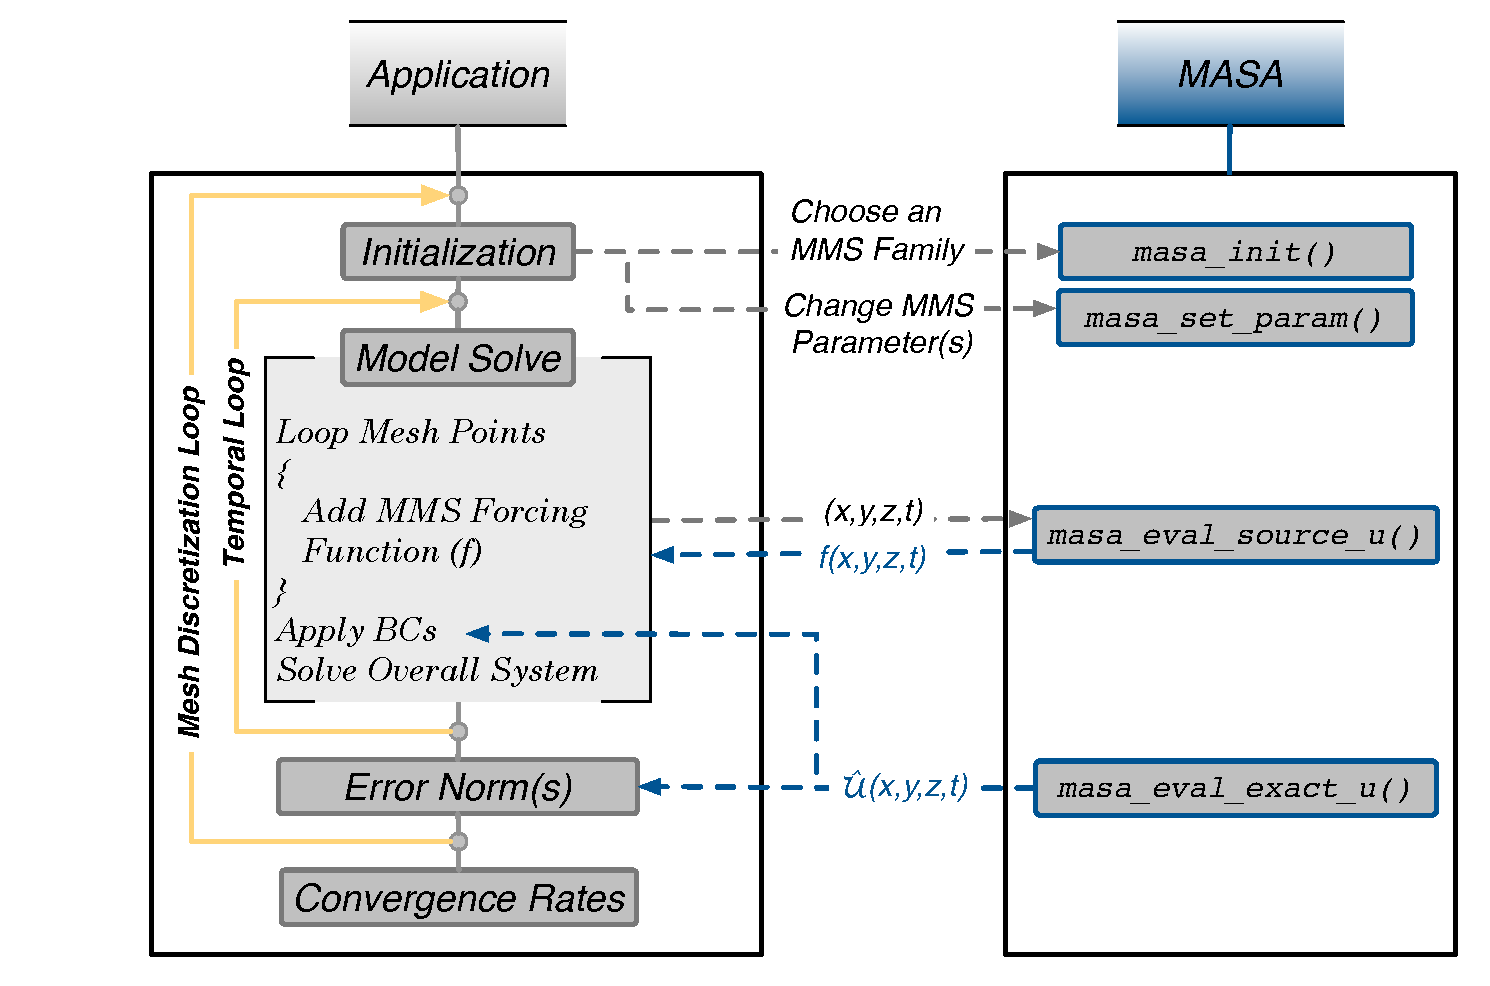
\includegraphics[width=.8\linewidth]{masa_overview} \\
  \end{center}
\end{frame}


%===============================================================================
% application linkage
%===============================================================================
\begin{frame}[fragile]
\frametitle{Fortran 90: What you need from MASA}
{\tiny
\begin{verbatim}
program main
  use masa
  implicit none

  dx = real(lx)/real(nx)
  dy = real(ly)/real(ny);

  ! initialize the problem
  call masa_init("laplace example","laplace_2d")

  ! evaluate source terms (2D)
  do i=0, nx
     do j=0, ny
         
        y = j*dy        
        x = i*dx
        
        ! evalulate source term
        field = masa_eval_2d_source_f   (x,y)

        ! evaluate analytical term
        exact_phi = masa_eval_2d_exact_phi (x,y)

     enddo
  enddo

end program main

\end{verbatim}
}
\end{frame}

%===============================================================================
% MASA API demo
%===============================================================================
\begin{frame}[fragile]
\frametitle{C: What you need from MASA}
{\tiny
\begin{verbatim}
#include <masa.h>

int main()
{
  err += masa_init("laplace example","laplace_2d");

  // grab / set parameter values
  Lx = masa_get_param("Lx");
  masa_set_param("Ly",42.0);

  for(int i=0;i<nx;i++)
    for(int j=0;j<nx;j++)
      {  
        x=i*dx;
        y=j*dy;

        // source term
        ffield    = masa_eval_2d_source_f (x,y);

        // manufactured solution
        phi_field = masa_eval_2d_exact_phi(x,y);

       } // finished iterating over space
} //end program
\end{verbatim}
}
\end{frame}

%===============================================================================
% NEW SLIDE: Python
%===============================================================================

\begin{frame}[fragile]
\frametitle{Python: What you need from MASA}
{\tiny
\begin{verbatim}

#
# import .libs relative path for masa.py
#
import os, sys
import numpy as np
lib_path = os.path.abspath('../src/.libs')
sys.path.append(lib_path)
import _masa

err  = 0
err += _masa.masa_init("laplace example","laplace_2d")

space = np.linspace(0,1.0,num=5)
for x in np.nditer(space):
    for y in np.nditer(space):
        ffield    = _masa.masa_eval_2d_source_f(x,y)
        phi_field = _masa.masa_eval_2d_exact_phi(x,y)


if(err == 0):
    # Steady as she goes
    sys.exit(0)
else:
    # something is wrong
    sys.exit(1)

\end{verbatim}
}
\end{frame}

%===============================================================================
% NEW SLIDE: future work
%===============================================================================

%===============================================================================
% idea: what if we change this to read about other possible physics/econ/stuff
%===============================================================================

\begin{frame}
  \frametitle{Future Solution Development}

  \begin{block}{Single Physics}
    \begin{itemize}
    \item Additional RANS models ($v^2$-f, k-$\epsilon$, etc.)
    \item Shocks
    %\item Thermochemical relaxation    
    \end{itemize}
  \end{block}

  \begin{block}{Stochastic PDEs}    
    \begin{itemize}
     \item Conjugate Priors
     \item Fokker-Plank (time evolution of pdfs)
     \item How do you verify something that is random?
    \end{itemize}
  \end{block}

  \begin{block}{Different physical systems}
    \begin{itemize}
    \item Einstein's field equations (General Relativity)
    \item Schrodinger equation (Quantum Mechanics)
    \item Black-Scholes (Finance)
    \item etc.
    \end{itemize}
  \end{block}

\end{frame}

%===============================================================================
% importing new solutions
%===============================================================================

\begin{frame}
  \frametitle{Importing New Solutions}

\begin{block}{Requirements}
  \begin{itemize}
  \item Latex documents can be loaded directly into MASA documentation
    \begin{itemize}    
      \item Model document detailing analytical solution and source terms
      \item Interface documentation detailing parameters and functions
    \end{itemize}
  \item Source and analytical terms in C/C++/Fortran90
    \begin{itemize}    
     \item Can be integrated into your local MASA copy automagically (perl!)
     \item Submit a patch
     \begin{itemize}    
      \item (unit tests would be nice)
     \end{itemize}
    \end{itemize}
   \item \textcolor{red}{Willingness to share}
   \item Publish these solutions!
  \end{itemize}
\end{block}

\begin{block}{}
  \begin{itemize}
    \item Success of MASA depends on use as a community tool
  \end{itemize}
\end{block}

\end{frame}

\begin{frame}
\frametitle{Shortcomings}

\begin{block}{Symbolic Shortcomings}
 \begin{itemize}
  \item Even with factorization, source terms still massive
  \item Generating manufactured solutions was a {\bf full time job} at PECOS
  \item Everything we have discussed has been generated outside of MASA
	\begin{itemize}
	 \item Not thrilled with Maple, Mathematica
	\end{itemize}
 \end{itemize}
\end{block}

 \begin{block}{Enter Automatic Differentiation}
  \begin{itemize}
   \item AD numerically evaluates the derivative of a function 
	\begin{itemize}
	 \item applies chain rule repeatedly 
	\end{itemize}
   \item Superior error characteristics (round-off)
   \item Slow (but we barely care)
   \item Several libraries: NAG, Sacado, etc.
  \end{itemize}
 \end{block}
\end{frame}

%===============================================================================
% NEW SLIDE: euler in masa
%===============================================================================
\begin{frame}[fragile]
\frametitle{MASA PDE Examples}

\begin{block}{Source Terms: Euler}
\begin{semiverbatim}
\footnotesize
\comment{// Arbitrary manufactured solutions}
\var{U}.\key{template} \func{get}<\data{0}>() = \var{u_0} + \var{u_x} * \func{sin}(\var{a_ux} * \var{PI} * \var{x} / \var{L}) 
                          + \var{u_y} * \func{cos}(\var{a_uy} * \var{PI} * \var{y} / \var{L}); 
\end{semiverbatim}

 \begin{center}
  $\nabla \cdot (\rho u ) = 0$ \\
  \vspace{15pt}
  $\nabla \cdot (e u) + p \nabla \cdot u = 0$
  \end{center}
\begin{semiverbatim}
\footnotesize

\comment{// Mass, momentum and energy}
\type{Scalar}   \var{Q_rho}   = \func{raw_value}(\func{divergence}(\var{RHO}*\var{U}));
\type{RawArray} \var{Q_rho_u} = \func{raw_value}(\func{divergence}(\var{RHO}*\var{U}.\func{outerproduct}(\var{U})) +
                   \var{P}.\func{derivatives}());
 \type{Scalar}  \var{Q_rho_e} = \func{raw_value}(\func{divergence}((\var{RHO}*\var{ET}+\var{P})*\var{U}));

\end{semiverbatim}
\end{block}
\end{frame}

%===============================================================================
% NEW SLIDE: future work
%===============================================================================

\begin{frame}
  \frametitle{Future AD work}

 \begin{block}{Future Work}
  \begin{itemize}
   \item Automatic Latex Generation
   \item Latex Parser -- MMS generator
   \item Will this work with complex multiphysics?
  \end{itemize}
 \end{block}
 
\end{frame}

%===============================================================================
% NEW SLIDE: Lab Collaboration
%===============================================================================
\begin{frame}
  \frametitle{SMASA: Stochastic MASA}

  \begin{block}{State-of-the-Art}
    \begin{itemize} 
    \item Verification of Bayesian model calibration algorithms
    \item Uses non-deterministic linear regression model:
    \end{itemize}
    
    \begin{equation*}
        y = G \beta + \epsilon(\lambda,\phi)
    \end{equation*}
    
    \begin{itemize}
      \item $y$ observations, G response matrix, $\beta$ unknowns, $\epsilon$ noise 
      \item Three cases: calibrations of $\beta, \lambda$ and $\phi$
      \item Two forms of priors: non-informative (Jeffreys) and Gaussian
    \end{itemize}
  \end{block}


    \centering
    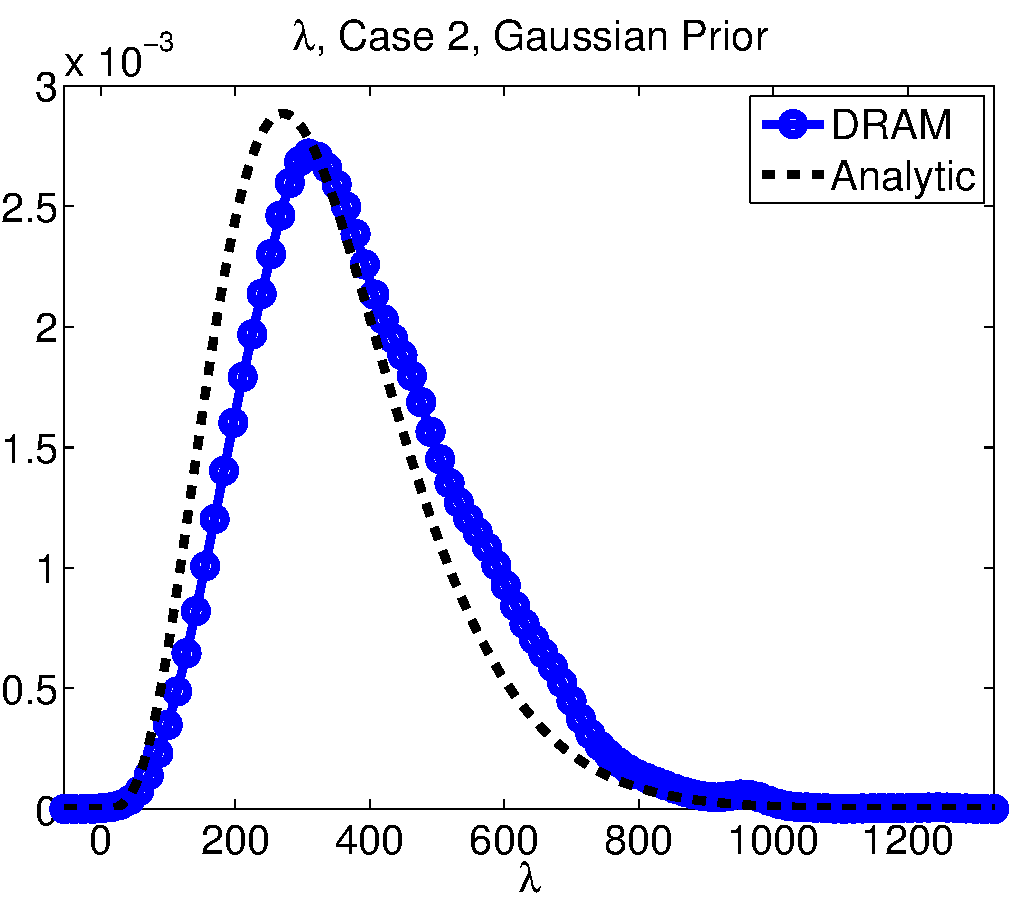
\includegraphics[scale=0.15]{smasa}

\end{frame}

%===============================================================================
% NEW SLIDE: Lab Collaboration
%===============================================================================
\begin{frame}
  \frametitle{Snapshot}

  \begin{block}{Release}
    \begin{itemize} 
    \item MASA 0.44.0 current release
    \item \url{https://github.com/manufactured-solutions/MASA}
    \item Open source, LGPL V2.1, free
    \end{itemize}
  \end{block}

  \begin{block}{Publications}
   \begin{itemize}
    \item ``MASA: a library for verification using manufactured
	  analytical solutions''
    \begin{itemize}
     \item DOI: 10.1007/s00366-012-0267-9
    \end{itemize}
    \small
   \item A TRANSIENT MANUFACTURED SOLUTION FOR THE COMPRESSIBLE NAVIER-STOKES EQUATIONS WITH A POWER LAW VISCOSITY
   \item Manufactured Solutions for the Favre-Averaged Navier-Stokes Equations with Eddy-Viscosity Turbulence Models
   \item ``A Linear Regression Framework for the Verification of Bayesian Model Calibration Algorithms'' (in prep)

   \end{itemize}
  \end{block}

\end{frame}

%===============================================================================
% finis
%===============================================================================
 \begin{frame}
   \frametitle{Conclusions}

   \begin{block}{Summary}
     \begin{itemize}
      \item MMS is not a difficult concept, but can be tricky and time
	    consuming 
      \item Must have a high degree of confidence in your verification suite
      \item MASA is an open source library designed to:
	    \begin{itemize}
	     \item Increase use of existing MMS in the community
	     \item Provide a standardized interface and toolset to the
		   community
	     \item Serve as an example of high quality verification
		   software
	    \end{itemize}
     \end{itemize}
   \end{block}
 \end{frame}

 \begin{frame}
   \frametitle{Conclusions}

   \begin{block}{}
    \begin{center}
     Thank you!
    \end{center}
    \center{Have a well verified day.} \\
    \center{nick@ices.utexas.edu}
    \end{block}

   \centering
   \includegraphics[scale=0.25]{eunuch}

 \end{frame}

%===============================================================================
% NEW SLIDE: finis
%===============================================================================

%===============================================================================
% combinatorial explosion
%===============================================================================

\begin{frame}
\frametitle{Combinatorial Explosion}

\begin{block}{Explosion in source term size}
  \begin{itemize}
  \item Complexity increases with more sophisticated mathematical models 
    \begin{itemize}
    \item Sutherland viscosity model has over 1,612,000 characters
    \end{itemize}
  \item Large memory requirements (128 GB not sufficient for Sutherland)
  \item Computational intensity
  \item \textcolor{orange}{segfaults}
  \end{itemize}
\end{block}

\begin{block}{Hierarchic MMS}
  \begin{itemize}
  \item Decompose each equation into sub-terms
  \item Each term is operated on individually to plug in a
    manufactured solution
  \item Resulting expressions are re-combined to regain source term
  \end{itemize}
\end{block}

\end{frame}

%===============================================================================
% Hierarchic MMS
%===============================================================================
\begin{frame}
\frametitle{The Hierarchic MMS}
\small
Consider the full 3D Navier-Stokes energy equation:
\begin{equation}
  \nonumber  
    \Lo= \Diff{\rho e_t}{t}+\nabla \cdot (\rho\mathbf{u}e_t) +\nabla\cdot \mathbf{q} +  \nabla\cdot(p  \mathbf{u}) - \nabla \cdot (\bv{\tau} \cdot \mathbf{u})
\end{equation}

  \begin{columns}[c]

    \begin{column}{4cm}
      Decompose:
      \begin{equation} 
        \begin{split}
          \nonumber
          \textcolor{red}{\Lo_1}&= \Diff{\rho e_t}{t} \\
          \Lo_2&=\nabla \cdot (\rho\mathbf{u}e_t) \\
          \textcolor{orange}{\Lo_3}&=\nabla\cdot \mathbf{q} \\
          \Lo_4&= \nabla\cdot(p  \mathbf{u}) \\
          \textcolor{blue}{\Lo_5}&=- \nabla \cdot (\bv{\tau} \cdot \mathbf{u})
        \end{split}
      \end{equation}
    \end{column}

    \begin{column}{7.5cm}
      \begin{block}{\small Hierarchic MMS extensions:}
        \begin{itemize}
          \small
          \item Expand each component of divergence
          \item Transient and steady cases ($\textcolor{red}{\Lo_1}$ = 0)
          \item Sutherland model only requires altering \textcolor{blue}{$\Lo_5$}
          \item Navier-Stokes $\rightarrow$ Euler and \textcolor{blue}{additional} \textcolor{orange}{terms}
        \end{itemize}        
      \end{block}
    \end{column}       
  \end{columns}
  \normalsize
\end{frame}

%===============================================================================
% hierarchic mms
%===============================================================================
\begin{frame}
  \frametitle{Hierarchic MMS Results}
  \begin{block}{Reductions}
    \begin{itemize}
    \item Symbolic factorization tricks permit further simplification of these operators:
      \newline
      \begin{table}[htb]
        \centering
        \begin{tabular}{c c c c}
          \hline
          Term & Before & After & Reduction\\
          \hline \vspace{-8pt} \\
          $\Lo_1$ & $70.1 \times 10^3$ & $1.1 \times 10^3$ & 98.4\%\\ 
          $\Lo_2$ & $292.8\times 10^3$ & $4.0 \times 10^3$ & 98.6\%\\ 
          $\Lo_3$ & $11.3 \times 10^3$ & $1.2 \times 10^3$ & 89.3\%\\
          $\Lo_4$ & $1.5\times 10^3$   & $5.8 \times 10^2$ & 61.3\%\\
          $\Lo_5$ & $3.1  \times 10^3$ & $1.3 \times 10^3$ & 58.0\%\\
          $\Lo  $ & $378.8\times 10^3$ & $8.2 \times 10^3$ & \textcolor{blue}{97.8\%} \\[.5ex]
          \hline
        \end{tabular}
        \label{table_charac}
      \end{table}

    \end{itemize}
  \end{block}

\end{frame}

%===============================================================================
% hierarchic mms
%===============================================================================
\begin{frame}
  \frametitle{Reduced source term C-output}
  \vspace{-15pt}
  \hspace{-1cm}\quad
  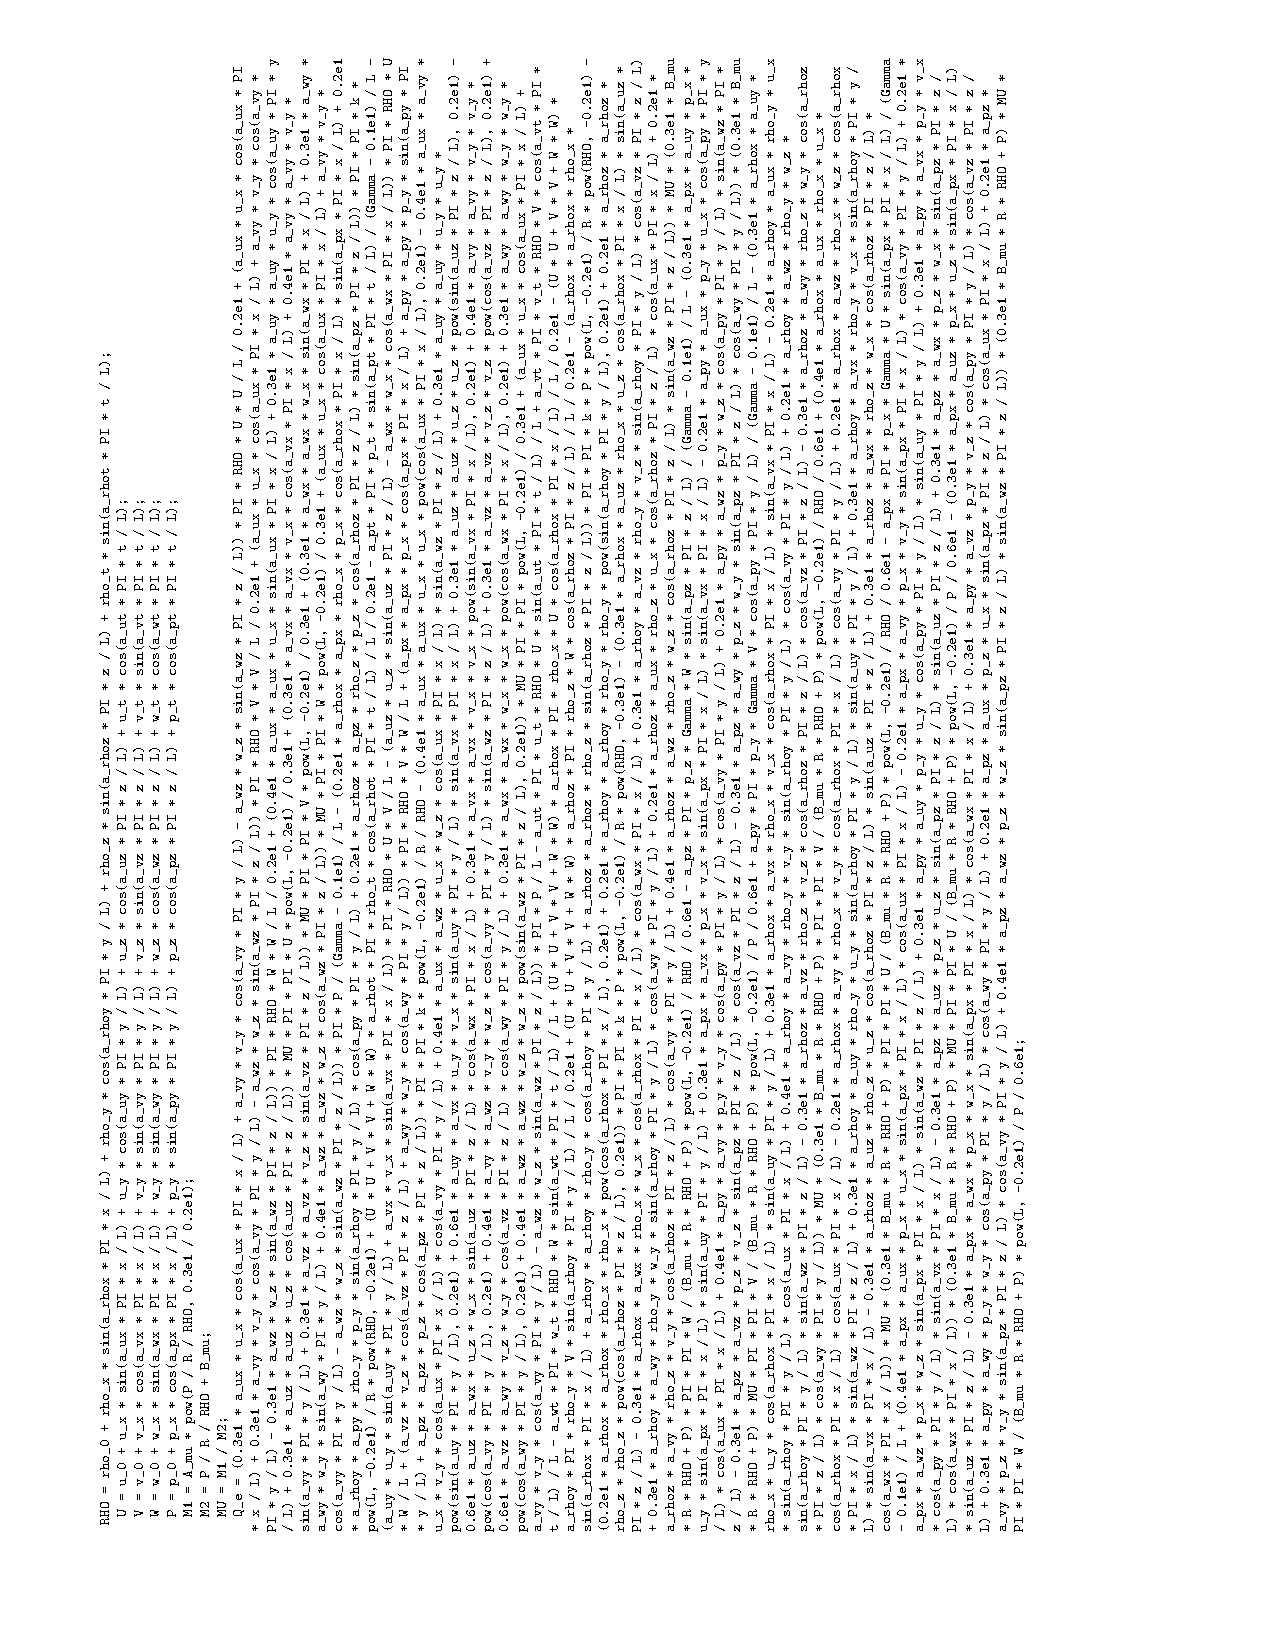
\includegraphics[scale=0.40]{EnergySutherland_3d}
\end{frame}

%===============================================================================
% reduction size
%===============================================================================

\begin{frame}
  \frametitle{Original source term C-output}
  \vspace{-15pt}
  \hspace{-1cm}\quad
  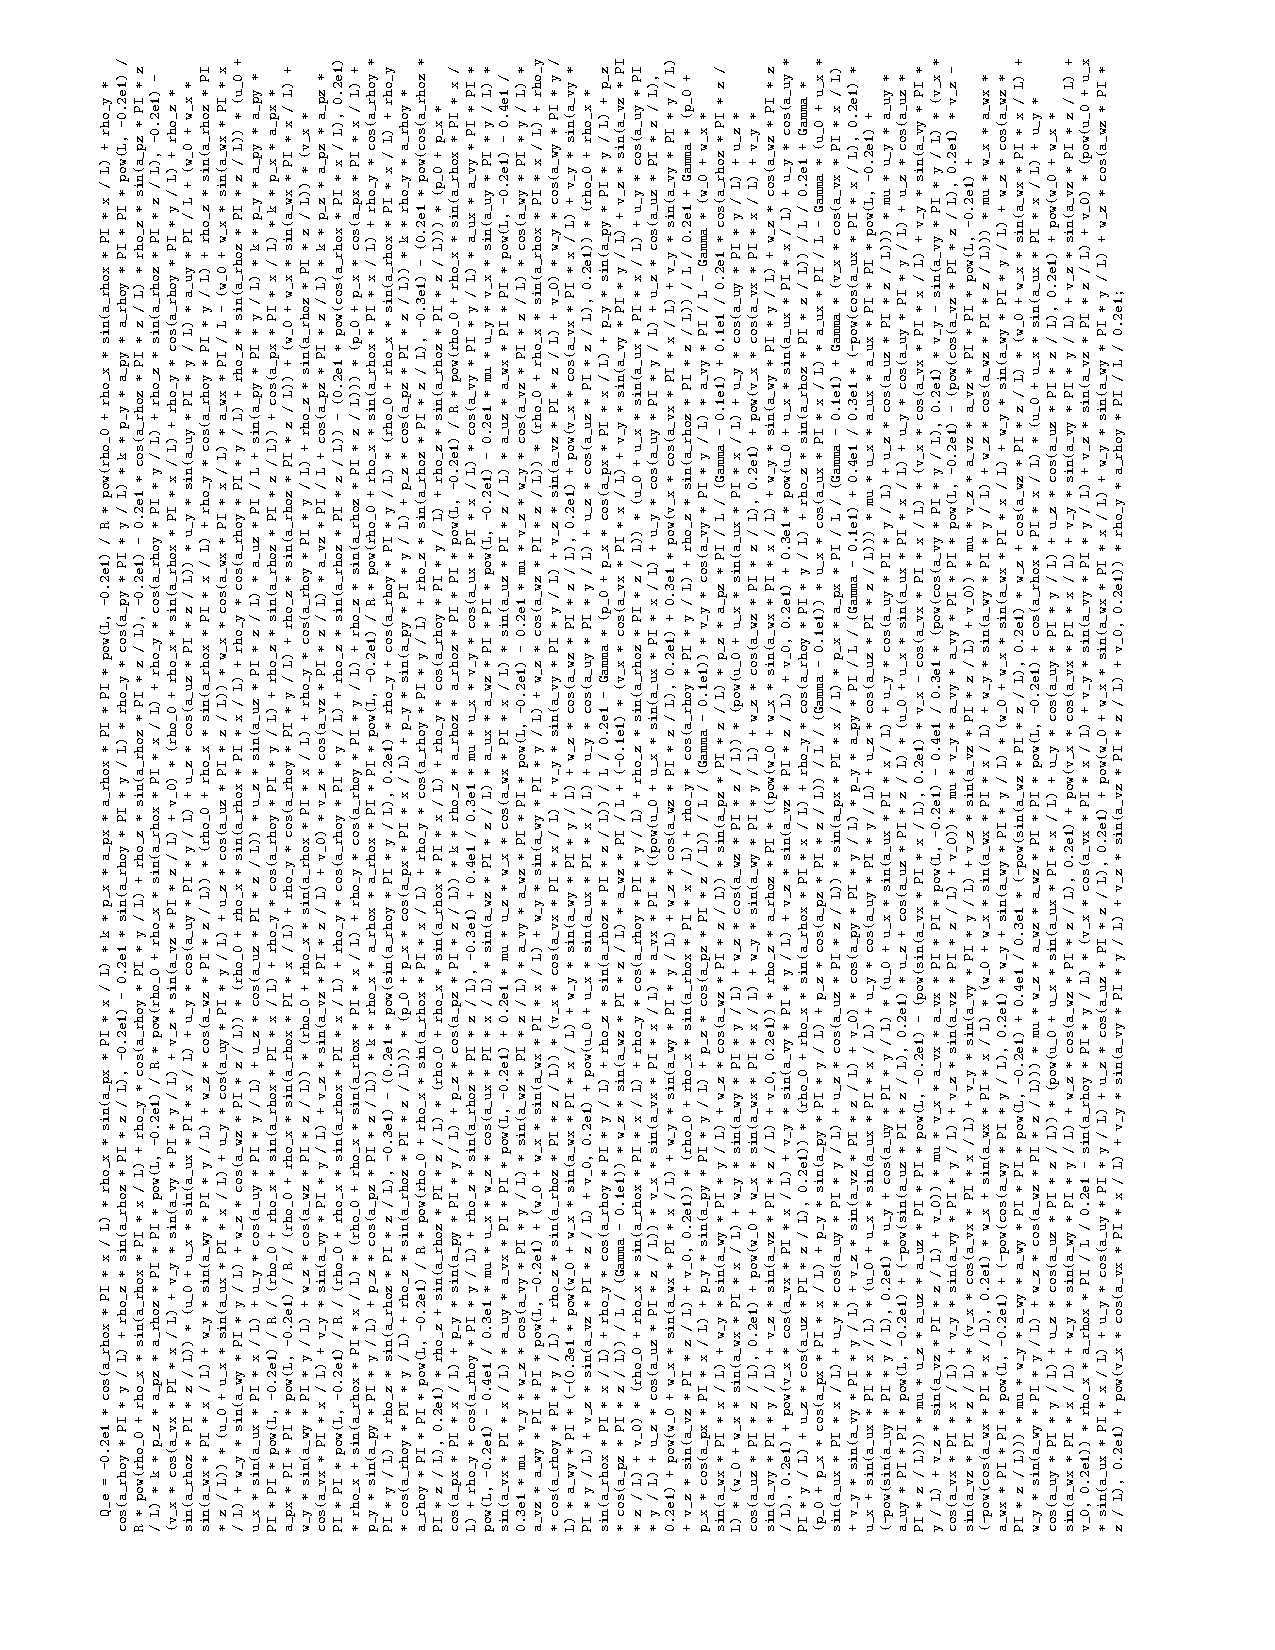
\includegraphics[scale=0.40]{Energy_3d_5}
\end{frame}

%===============================================================================
% NEW SLIDE: transition to AD
%===============================================================================
\begin{frame}
\frametitle{Shortcomings}

\begin{block}{Symbolic Shortcomings}
 \begin{itemize}
  \item Hierarchic decomposition is an improvement, but is it enough?
	\begin{itemize}	 
	 \item Even with factorization, source terms still massive
	 \item Generating manufactured solutions was a {\bf full time job} at PECOS
	\end{itemize}
  \item Everything we have discussed has been generated outside of MASA
	\begin{itemize}
	 \item Not thrilled with Maple, Mathematica
	\end{itemize}
 \end{itemize}
\end{block}

\begin{block}{Enter Automatic Differentiation}
 \begin{itemize}
  \item AD numerically evaluates the derivative of a function 
	\begin{itemize}
	 \item applies chain rule repeatedly 
	\end{itemize}
  \item Superior error characteristics (round-off)
  \item Slow (but we barely care)
  \item Several libraries: NAG, Sacado, etc.
 \end{itemize}
\end{block}
\end{frame}

%===============================================================================
% NEW SLIDE: complex numbers
%===============================================================================
\begin{frame}
\frametitle{Review: Complex Numbers}

\begin{itemize}
\item A new element $i$

\item Take the quotient with $i^2 \equiv -1$
\[\Complex[\Reals] \equiv \left\{a + b i: a,b \in \Reals\right\}\]
\item Arithmetic:
\end{itemize}
\begin{align*}
(a+b i) + (c+d i) &= ((a+c) + (b+d) i) \\
(a+b i) - (c+d i) &= ((a+c) - (b+d) i) \\
(a+b i) \times (c+d i) &= (ac) + ad i + bc i + bd i^2 \\
                              &= ((ac) + (ad+bc)i - (bd))
\end{align*}
\end{frame}


%===============================================================================
% NEW SLIDE: AD dual numbers
%===============================================================================
\begin{frame}
\frametitle{``Dual Numbers'' - [Clifford 1873],[Study 1891]} 

\begin{itemize}
\item A new element $\epsilon$
\item Closed under addition and multiplication:
\[\left\{\sum_{i=0}^{m} a_i \epsilon^i: a_i \in \Reals, m < \infty\right\}\]
\item Take the quotient with $\epsilon^2 \equiv 0$
\[\Duals[\Reals] \equiv \left\{a + b \epsilon: a,b \in \Reals\right\}\]
\item Used with quaternions to represent rotations and translations
\item Arithmetic:
\end{itemize}
\begin{align*}
(a+b\epsilon) + (c+d\epsilon) &= ((a+c) + (b+d)\epsilon) \\
(a+b\epsilon) - (c+d\epsilon) &= ((a+c) - (b+d)\epsilon) \\
(a+b\epsilon) \times (c+d\epsilon) &= (ac) + ad\epsilon + bc\epsilon + bd\epsilon^2 \\
                              &= ((ac) + (ad+bc)\epsilon)
\end{align*}
\end{frame}

%===============================================================================
% NEW SLIDE: hyperdual
%===============================================================================
\begin{frame}
\frametitle{``Hyper-dual Numbers'' - [Fike 2009]}

\begin{itemize}
\item Add two new elements $\epsilon_1$, $\epsilon_2$ to $\Reals$
\item Take the quotient with $\epsilon_1^2 \equiv \epsilon_2^2 \equiv 0$
\[\Hyperduals[\Reals] \equiv \left\{a + b \epsilon_1 + c \epsilon_2 + d \epsilon_1 \epsilon_2: a,b,c,d \in \Reals\right\}\]
\item Arithmetic:
\end{itemize}
\begin{align*}
(a+b\epsilon_1+c\epsilon_2+d\epsilon_1 \epsilon_2) + 
  (e+f\epsilon_1+g\epsilon_2+h\epsilon_1 \epsilon_2) &= \\
  ((a+e) + (b+f)\epsilon_1 + (c+g)\epsilon_2 + (d+h)\epsilon_1 \epsilon_2) & \\
(a+b\epsilon_1+c\epsilon_2+d\epsilon_1 \epsilon_2) - 
  (e+f\epsilon_1+g\epsilon_2+h\epsilon_1 \epsilon_2) &= \\
  ((a-e) + (b-f)\epsilon_1 + (c-g)\epsilon_2 + (d-h)\epsilon_1 \epsilon_2) & \\
(a+b\epsilon_1+c\epsilon_2+d\epsilon_1 \epsilon_2) \times
  (e+f\epsilon_1+g\epsilon_2+h\epsilon_1 \epsilon_2) &= \\
(ae) + (af+be)\epsilon_1 + (ag+ce)\epsilon_2 + (ah+de+bg+cf)\epsilon_1\epsilon_2 & 
\end{align*}

\end{frame}

%===============================================================================
% NEW SLIDE
%===============================================================================
\begin{frame}
\frametitle{``Hyper-Dual Numbers''}
 \begin{itemize}
  \item With $\epsilon_1^2 \equiv \epsilon_2^2 \equiv 0 \equiv (\epsilon_1
	\epsilon_2)^2 = 0$
	
  \item Where $X \equiv x + \epsilon_1 + \epsilon_2$, we find:
 \end{itemize}
 \[ f(X) = f(x) + f'(x) \epsilon_1 + f'(x) \epsilon_2 + f''(x) \epsilon_1 \epsilon_2 \]

 \begin{itemize}
  \item The Taylor series truncates exactly at the second-derivative term
  \item Using hyper-dual numbers results in first- and second-derivative
	calculations that are exact, regardless of step size
  \item Methods for computing exact higher derivatives can be created by
	using more non-real parts ($\epsilon_3$, for instance)
  \begin{itemize}
   \item Accomplished using Templates in C++
  \end{itemize}
 \end{itemize}
\end{frame}

\end{document}
